\documentclass[11pt,]{article}
\usepackage[]{mathpazo}
\usepackage{amssymb,amsmath}
\usepackage{ifxetex,ifluatex}
\usepackage{fixltx2e} % provides \textsubscript
\ifnum 0\ifxetex 1\fi\ifluatex 1\fi=0 % if pdftex
  \usepackage[T1]{fontenc}
  \usepackage[utf8]{inputenc}
\else % if luatex or xelatex
  \ifxetex
    \usepackage{mathspec}
  \else
    \usepackage{fontspec}
  \fi
  \defaultfontfeatures{Ligatures=TeX,Scale=MatchLowercase}
\fi
% use upquote if available, for straight quotes in verbatim environments
\IfFileExists{upquote.sty}{\usepackage{upquote}}{}
% use microtype if available
\IfFileExists{microtype.sty}{%
\usepackage{microtype}
\UseMicrotypeSet[protrusion]{basicmath} % disable protrusion for tt fonts
}{}
\usepackage[margin = 1in]{geometry}
\usepackage{hyperref}
\hypersetup{unicode=true,
            pdftitle={Saved by the pulse? Separating the effects of total and temporal food abundance on the performance of bumble bee microcolonies},
            pdfauthor={Jeremy Hemberger; Agathe Frappa; Grant Witynski; Claudio Gratton},
            pdfkeywords={\emph{Bombus impatiens}, colony growth, floral resources, temporal
variability, agroecosystems},
            pdfborder={0 0 0},
            breaklinks=true}
\urlstyle{same}  % don't use monospace font for urls
\usepackage{graphicx,grffile}
\makeatletter
\def\maxwidth{\ifdim\Gin@nat@width>\linewidth\linewidth\else\Gin@nat@width\fi}
\def\maxheight{\ifdim\Gin@nat@height>\textheight\textheight\else\Gin@nat@height\fi}
\makeatother
% Scale images if necessary, so that they will not overflow the page
% margins by default, and it is still possible to overwrite the defaults
% using explicit options in \includegraphics[width, height, ...]{}
\setkeys{Gin}{width=\maxwidth,height=\maxheight,keepaspectratio}
\IfFileExists{parskip.sty}{%
\usepackage{parskip}
}{% else
\setlength{\parindent}{0pt}
\setlength{\parskip}{6pt plus 2pt minus 1pt}
}
\setlength{\emergencystretch}{3em}  % prevent overfull lines
\providecommand{\tightlist}{%
  \setlength{\itemsep}{0pt}\setlength{\parskip}{0pt}}
\setcounter{secnumdepth}{0}
% Redefines (sub)paragraphs to behave more like sections
\ifx\paragraph\undefined\else
\let\oldparagraph\paragraph
\renewcommand{\paragraph}[1]{\oldparagraph{#1}\mbox{}}
\fi
\ifx\subparagraph\undefined\else
\let\oldsubparagraph\subparagraph
\renewcommand{\subparagraph}[1]{\oldsubparagraph{#1}\mbox{}}
\fi

%%% Use protect on footnotes to avoid problems with footnotes in titles
\let\rmarkdownfootnote\footnote%
\def\footnote{\protect\rmarkdownfootnote}

%%% Change title format to be more compact
\usepackage{titling}

% Create subtitle command for use in maketitle
\providecommand{\subtitle}[1]{
  \posttitle{
    \begin{center}\large#1\end{center}
    }
}

\setlength{\droptitle}{-2em}

  \title{Saved by the pulse? Separating the effects of total and temporal food
abundance on the performance of bumble bee microcolonies}
    \pretitle{\vspace{\droptitle}\centering\huge}
  \posttitle{\par}
    \author{Jeremy Hemberger \\ Agathe Frappa \\ Grant Witynski \\ Claudio Gratton}
    \preauthor{\centering\large\emph}
  \postauthor{\par}
      \predate{\centering\large\emph}
  \postdate{\par}
    \date{April 29, 2019}

\usepackage{setspace}

\doublespacing
\usepackage[left]{lineno}
\linenumbers
\usepackage{dcolumn}
\usepackage{caption}
\usepackage{float}
\usepackage{afterpage}

\begin{document}
\maketitle
\begin{abstract}
The loss of flower-rich habitat to agriculture is a key factor
contributing to bumble bee declines across Europe and North America.
Yet, agricultural intensification has not only altered flower abundance
in the landscape, but also affected when flowers are available during
the season (e.g., mass-flowering crops). While we know that both total
pollen and nectar as well as temporal availability can impact bumble bee
colony success (growth and reproductive output), we have yet to
understand how these two factors combined might manifest. We designed an
experiment to decouple the effects of total food abundance and its
temporal availability on bumble bee microcolony development, by exposing
them to either constant or pulsed food availability at two ration
levels, 100\% and 60\% ad-libitum food abundance. Microcolonies provided
constant, full-rations of food grew the most, while those fed variable,
full-rations struggled to gain mass. Regardless of temporal
presentation, microcolonies fed 60\% ad-libitum rations gained little
mass over the experiment. Reproductive output was greatest in
microcolonies fed full-rations, regardless of the temporal availability
of food, while those given 60\% rations struggled to produce numerous
drones. This study highlights the importance of flower abundance in
agricultural landscapes for both colony growth and reproduction, and
suggests that increasing flower abundance could lead to improved colony
fitness.
\end{abstract}

\hypertarget{introduction}{%
\section{Introduction}\label{introduction}}

Bumble bee declines across Europe and North America are driven by a
number of interacting anthropogenic factors (e.g., pesticides, McArt et
al. 2017), novel diseases from managed bees (Brown et al. 2016; Fürst et
al. 2014) and climate change (Kerr et al. 2015)). There is a growing
consensus that habitat loss is the most important driver of decline
(Roulston and Goodell 2011; Senapathi et al. 2015; Goulson and Nicholls
2016). In the US Midwest, two centuries of agricultural intensification
(defined here as the spatially extensive increase of agrichemical use
and proliferation of monocultures (e.g., Benton, Vickery, and Wilson
2003) has removed bumble bee habitat - supplanting once continuous
landscapes of prairie, savanna, and wetlands with highly productive
agricultural crops (Smith 1998; Rhemtulla, Mladenoff, and Clayton 2007).
Coincident with the transition to primarily agricultural land use in the
US, several species of bumble bee have declined precipitously (Grixti et
al. 2009; Cameron et al. 2011; Jacobson et al. 2018).

Most importantly, agricultural intensification has led to wholesale
change in the abundance and temporal availability of floral resources in
the landscape (Goulson 2010; Schellhorn, Gagic, and Bommarco 2015;
Goulson et al. 2015; Vaudo et al. 2018). Historically, landscapes
containing a continuous supply of diverse floral resources (e.g.,
tall-grass prairies (Hines and Hendrix 2005)) were prolific, however
many of these landscapes have been lost to commodity agriculture (Smith
1998). Contemporary commodity crop landscapes in the Midwest (e.g., corn
and soy), featuring decreased crop diversity in combination with an
increased use of herbicides, have significantly reduced flowering plant
availability (Carvell et al. 2006; Goulson et al. 2015), creating
proverbial food deserts for bumble bees aside from small patches of
remnant natural habitat. In contrast, some agricultural landscapes
contain mass-flowering crops (e.g., fruit crops, canola) that provide
large pulses of floral resources, albeit over a short time period
(Westphal, Steffan-Dewenter, and Tscharntke 2009; Holzschuh et al. 2013;
Rundlöf et al. 2014). As such, with respect to floral resource
abundance, a range of possible landscapes exist in agriculturally
dominated regions. However, the trend has moved toward highly simplified
landscapes, with floral resources available only during crop bloom.

The interaction between total floral resource abundance and temporal
availability in the landscape can be visualized conceptually, as two
potentially independent factors (Fig.1). In this abstraction, `Zone 1'
landscapes contain few flowers that are constantly available over the
course of the growing season. This can be contrasted with `Zone 3'
landscapes that contain an abundance of flowers, but primarily only
during two pulses (e.g., two mass-flowering crops). This framework
allows us to make simple predictions of how bumble bees are likely to
respond to changes in floral resource abundance in the landscape. We
might expect, given that bumble bees are obligate flower visitors
existing in long-lived colonies, that access do an abundance of flowers
that are consistently available over time (e.g., `Zone 2' landscapes)
would be critical for successful colony development.

Total floral resource abundance is an important factor that contributes
to the growth and reproductive success of bumble bee colonies. For
example, worker production is dependent on pollen and nectar influx to
the colony; shortfalls can be detrimental to worker output (Williams,
Regetz, and Kremen 2012; Cartar and Dill 1991; Sutcliffe and Plowright
1988), and reproductive (drone and gyne) output can be enhanced with
increased food availability (Pelletier and McNeil 2003). Despite
variable effect sizes and experimental methodologies, most studies tend
to agree that increased flower abundance leads to increased bumble bee
abundance (e.g., Carvell et al. 2007; Blaauw and Isaacs 2014) and/or
colony performance (e.g., Spiesman et al. 2017).

While total food availability is key for developing bumble bee colonies,
when food is available can be equally important (Schellhorn, Gagic, and
Bommarco 2015). Because bumble bee colonies have three distinct
bottlenecks wherein food availability is crucial to colony success
(queen colony establishment, colony worker buildup, and reproductive
production), food shortages during any period of the colony life cycle
can impair colony function. As such, continuous availability of flowers
in the landscape is believed to be paramount for bumble bees (e.g.,
Fig1, Zone 2 Martins et al. 2018). Past work has examined the effect of
total food abundance (Rotheray, Osborne, and Goulson 2017) and temporal
availability (Schmid-Hempel and Schmid-Hempel 1998) on colony
development independently, however we have yet to test the interactive
effect of the two. Is a lack of food, the temporal availability of food,
or both limiting bumble bee colony success? Parsing these two
interacting factors apart could help explain specific mechanisms
underlying bumble bee declines in agricultural landscapes, as well as
suggest conservation interventions.

To decouple the effects of total food abundance and temporal
availability on bumble bee colony development, we designed a 2x2
factorial experiment that varied total food amount and its temporal
availability. Treatment designs were meant to simulate hypothetical
scenarios that provide bumble bees either constantly available, or
pulsed food resources at two ration levels: 100\% and 60\% ad-libitum
(ad-lib) (Fig.1). These may represent different modalities of food
intake corresponding to different types of agricultural landscapes. For
example, bumble bees might experience landscapes containing few floral
resources and only during one short period of time (e.g., Fig1, Zone 4)
or a landscape containing many floral resources that are consistently
available (e.g., Fig1, Zone 2).

Using microcolonies of the Common Eastern bumble bee (\emph{Bombus
impatiens} Cresson), we tested the following hypotheses: (1)
microcolonies provided 100\% ad-lib food (pollen and nectar) in
constant, equally sized rations would gain the most mass and have the
greatest reproductive output (e.g., zone 2); (2) microcolonies provided
100\% ad-lib in pulses separated by periods of relative starvation would
perform slightly worse compared to those provided 100\% ad-lib in equal
rations, as \emph{B impatiens'} population stability in agricultural
landscapes suggests resilience to land-use change and variability in
food quantity (Cameron et al. 2011; Grab et al. 2019); (3) microcolonies
provided 60\% ad-lib would perform worst, regardless of temporal
treatment (equal, ``zone 1'' vs.~pulse, ``zone 4'' rations), as colonies
would be too nutritionally stressed, regardless of relatively large,
episodic influxes of food in the pulsed colonies.

\hypertarget{materials-and-methods}{%
\subsection{Materials and methods}\label{materials-and-methods}}

\hypertarget{experimental-design-and-procedure}{%
\paragraph{Experimental design and
procedure}\label{experimental-design-and-procedure}}

To assess the impact of varying total, and temporal food abundance on
bumble bee colony production, we designed a 2x2 factorial experiment
utilizing microcolonies of \emph{B. impatiens}. Microcolonies were used
as proxies to full colonies given their ease of establishment and
well-documented analogs to full colony development (Tasei and Aupinel
2008; Dance, Botías, and Goulson 2017; Moerman et al. 2017).

In three experimental rounds, we established microcolonies from: (Round
1) 10 queen-right colonies sourced from Koppert Biological Systems
(Howell, MI) in February of 2018; (Round 2) 10 queen-right colonies from
Koppert Biological Systems in May of 2018; (Round 3) 10 queen-right
colonies sourced from BioBest Biological (Romulus, MI) in October of
2018. In each round, microcolony initiation was identical. We removed
sets of 5 workers from a random colony and placed sets into 28 acrylic
plastic microcolony rearing boxes (10 x 15 x 10 cm), provisioning each
with 2 grams of honey bee collected pollen homogenized with nectar and
sealed in honey bee wax, as well as ad-libitum nectar through a
sub-floor cotton wick and reservoir (ProSweet: MannLake LTD, Minnesota).
To allow microcolony initiation, we left colonies undisturbed for
approximately 1 week. Once we observed evidence of microcolony
establishment (egg and larval brood masses visible) in each replicate
box, we removed any remaining pollen and nectar, and initiated treatment
regimes. In order to ensure microcolonies had equal capacity to respond
to food availability (i.e., 5 workers per box), we replaced any deceased
workers throughout the experiment with randomly selected workers from
queen-right feeder colonies.

Over 8 weeks, we simulated landscape-scale food availability (both
pollen and nectar) in four treatments - each representing a hypothetical
landscape whereby total food abundance, and temporal availability were
independently altered according to the factorial design (Fig1).
Treatment conditions (hereafter, ``zones'') were as follows: ``Zone 1''
microcolonies were fed equal rations at 60\% ad-lib levels; ``Zone 2''
microcolonies were fed equal rations at 100\% ad lib levels; ``Zone 3''
microcolonies were fed in total the same amount of food as Zone 2
microcolonies, but food resources were provided as two large pulses with
periods of relative starvation (\textasciitilde{}60\% ad-lib)
encompassing the pulses; ``Zone 4'' microcolonies temporal availability
was the same as Zone 3, but with total food over the experiment equal to
Zone 1, and periods of relative starvation between pulses at
\textasciitilde{}38\% ad-lib. Seven microcolonies were randomly assigned
to each treatment. To determine total food rations supplied in each
treatment over the course of the experiment, we used measurements
reported in (Rotheray, Osborne, and Goulson 2017) (which reported on
ad-lib consumption rates of the ecological analog of \emph{B.
impatiens}, \emph{B. terrestris}), scaling total experiment food
abundance at 100\% ad-lib to 5 workers (approximately 33 grams of pollen
and 300 grams of nectar) over 17 feeding intervals (\textasciitilde{} 8
weeks). Reduced-ration treatments were scaled to 60\% of that value.

Every 3 days (hereafter interval feeding days: IFD), we massed whole
microcolonies by placing them on a scale and recording mass to the
nearest 0.01 grams. After massing, we fed microcolonies by providing an
appropriately massed pollen ball and nectar cup (see Supplemental
Material for feeding schedule and layout of microcolony box) depending
on the food treatment. After every 3 IFDs (every 9 Julian days), we
removed and massed the pollen that was not consumed in the microcolony
to calculate consumption. Nectar rations were replaced at every IFD -
each massed before addition and after removal to determine nectar
consumption (similar to Rotheray, Osborne, and Goulson 2017). We massed
the microcolony before the removal or addition of food to ensure that
measurements were comparable between IFDs.

To determine if treatments affected the relative fitness of each
microcolony, we censused colonies at each IFD. Censusing included
tallying worker mortality, drone (male) emergence, and presence of
different brood stages within the microcolony. After tallying drones
that had emerged, we removed and froze them for subsequent analysis. We
determined average drone wet mass per IFD for each microcolony,
individual drone intertegular distance (to nearest 0.01mm using ProgRes
CapturePro v2.0).

\hypertarget{data-analysis}{%
\paragraph{Data analysis}\label{data-analysis}}

We performed all data management and statistical analyses in R, version
3.5.1 (R Core Team 2019). For each colony, we calculated the estimated
``actual'' microcolony mass relative to IFD 1. The goal of this
calculation was to best determine how much biomass was being added to
the actual brood mass within the microcolony between IFDs while
factoring out added, but not consumed, food:

\[
\begin{aligned}
Estimated Brood Mass_{IFD = n} = Microcolony Mass_{IFD = n} - Microcolony Mass_{IFD = 1} + \\
Pollen Consumed_{IFD = n} - Pollen Added_{IFD = n}
\end{aligned}
\]

where \(Microcolony Mass_{IFD}\) is the mass of the entire microcolony
(including box) at \texttt{IFD\ =\ n}; \(Microcolony Mass_{IFD = 1}\) is
the mass of the entire microcolony on the first IFD: we calculated mass
gains relative the mass at IFD = 1; \(Pollen Consumed_{IFD = n}\) is the
average pollen consumed at \texttt{IFD\ =\ n}, determined by taking the
pollen consumed over the course of 3 IFDs (determined after removing
unconsumed pollen every 3 IFDs) and dividing by 3; and
\(Pollen Added_{IFD = n}\) is the mass of pollen added at at
\texttt{IFD\ =\ n} (see example calculation in Supplemental Material).
In the event that missing data prevented
\(Estimated Brood Mass_{IFD = n}\) from being determined (\textless{}
1\% of data), we interpolated the missing values using the
\texttt{na.approx} function from the R package \texttt{zoo} (Zeileis and
Grothendieck 2005). Nectar storage/consumption within the microcolony
was not considered for the \(Microcolony Mass_{IFD = n}\) calculation,
as we were not able to parse out nectar consumed by workers from nectar
moved by workers to honey pots in the brood mass. At the end of the
experiment, we also measured the mass of the brood cluster (including
all wax, remaining pupae, larvae, eggs, and nectar) alone after removing
them from the microcolony boxes.

To evaluate whether treatments affected end of experiment brood mass,
drone production, drone fitness parameters (wet mass and IT distance),
or worker mortality, we constructed linear mixed-effects models (LMMs)
on the combined data set from all three experimental rounds using the
\texttt{nlme} package (Pinheiro et al. 2018). Each model took the
general form of a given response variable as a function of treatment
(full-factorial between total food abundance and temporal variability)
and experimental round, with random intercept and slope estimates for
each microcolony. We estimated treatment means from LMMs (package:
\texttt{lsmeans} Lenth 2016) and used Tukey corrected pair-wise
comparisons (package: \texttt{multcomp} Hothorn, Bretz, and Westfall
2008) to determine significance between treatments. Additional contrasts
and effect sizes were calculated using the \texttt{emmeans} package
(Lenth 2019).

We also constructed repeated measures ANOVAs using the \texttt{nlme}
package to model colony mass, IFD average and cumulative drone
production, IFD average and cumulative worker mortality, as well as IFD
average and cumulative nectar and pollen consumption throughout the
course of the 8-week experiments. These models took the general form of
a given response as a function of treatment, date, and round, with a
random slope and intercept estimates for each microcolony. To account
for temporal autocorrelation, each analysis included a first order
autocorrelation structure (function: \texttt{corAR1}) with a time
covariate of measurement date and a grouping factor of colony identity.
We specified the autocorrelation correction using the lag = 1 value from
an identical model fitted with no autocorrelation structure.

Lastly, we calculated the growth rate of each microcolony for time
periods relative food pulses (Before pulse 1, during pulse 1, after
pulse 1 and before pulse 2, during pulse 2, and after pulse2). This was
accomplished by fitting a linear model of microcolony mass as a function
of IFD (time) for each replicate microcolony. We then extracted each
slope coefficient (i.e., the growth rate for a given microcolony during
an aforementioned time period) and constructed an ANOVA for each time
period to determine differences in growth rates among treatments, within
time periods. The \emph{P}-values associated with our initial slope
estimates (mass as a function of IFD) were used to test whether growth
was different than zero for a given time period. We also constructed a
repeated measures ANOVA for all slope estimates across all time periods
to determine if there were statistical differences in temporal
microcolony growth rates.

\hypertarget{results}{%
\subsection{Results}\label{results}}

\hypertarget{microcolony-establishment}{%
\paragraph{Microcolony establishment}\label{microcolony-establishment}}

Overall, microcolony establishment success was high across experimental
rounds, with only 3 of 84 failing to initiate (96\% success). Two
additional microcolonies contained a hyper-aggressive worker that killed
all original and replacement nest-mates when establishing dominance.
Despite increased aggression, these single-worker colonies still
produced males. However, we removed them from analyses as the response
of a single-worker microcolony to treatments was not comparable to
standard, five-worker microcolonies.

\hypertarget{microcolony-growth-mass-and-food-consumption}{%
\paragraph{Microcolony growth (mass and food
consumption)}\label{microcolony-growth-mass-and-food-consumption}}

The magnitude, and pattern of microcolony growth depended on treatment
throughout the course fo the experiment (Fig 2A,C). End of experiment
microcolony mass was driven by an interaction of both total food
abundance, as well as temporal availability (Fig 2B,D: interaction
effect, F\textsubscript{1,24} = 7.77, \emph{P} = 0.01). In the constant
ration treatments (zones 1 and 2), end of experiment mass for zone 2
microcolonies was, on average, 92\% greater than zone 1 microcolonies
(Fig 2B, t\textsubscript{24} = 5.33, \emph{P} \textless{} 0.001). In the
pulsed ration treatments (zones 3 and 4), end of experiment mass for
zone 3 microcolonies was, on average, 27\% more than zone 4
microcolonies, however the difference was not statistically clear (Fig
2D, t\textsubscript{24} = 1.77 , \emph{P} = 0.311). Average mass at the
end of the experiment for the two 100\% ad-lib treatments (zones 2 and
3) was 56\% greater for zone 2 relative to zone 3 (t = 4.37, \emph{P} =
0.001). There was a statistically clear effect of experimental round on
end of experiment mass, with rounds 2 and 3 overall weighing less at the
end of the experiment relative to round 1 (F\textsubscript{1,45} =
35.88, \emph{P} \textless{} 0.001). However, the pattern of end of
experiment mass across treatments was consistent between rounds
(F\textsubscript{1,45} = 3.18, \emph{P} = 0.081).

Microcolony growth rates over the course of the experiment varied by an
interaction of both total food abundance and temporal availability (Fig
3: F\textsubscript{1,24} = 12.13, \emph{P} = 0.002). Overall, zone 2
average growth rate was the highest (zone 2 effect: t\textsubscript{24}
= 5.06, \emph{P} \textless{} 0.001), while zone 1 growth rates were only
statistically above 0 during one time period (before pulse 1). Growth
rates were similar among pulsed-ration treatments. Both pulsed-ration
treatments experienced negative growth during periods following food
pulses (after pulse 1/before pulse2, after pulse 2). While mass gain was
negligible during the first pulse, it was greatest during the second
food pulse.

The effect of treatments on pollen consumption varied by experimental
round (F\textsubscript{2,41} = 5.72, \emph{P} = 0.006). Within
treatments, only total food abundance affected pollen consumption
(F\textsubscript{1,24} = 22.83, \emph{P} \textless{} 0.001), with
constant 100\% ration microcolonies consuming the most (Pollen: 14.80
+/- 0.813 grams). Zone 3 microcolony pollen consumption was not
significantly different than zones 1 and 4, despite a 40\% difference in
pollen availability over the course of the experiment. Nectar
consumption followed a similar pattern with consumption driven by total
abundance (Supplemental Fig2: F\textsubscript{1,24} = 60.98, \emph{P}
\textless{} 0.001), however there was no clear interactive effect of
experimental round (F\textsubscript{2,41} = 2.98, \emph{P} \textless{}
0.068).

\hypertarget{microcolony-demography-drone-production-and-worker-mortality}{%
\paragraph{Microcolony demography (drone production and worker
mortality)}\label{microcolony-demography-drone-production-and-worker-mortality}}

We found that total drone production increased with total food abundance
(Fig 4: F\textsubscript{1,24} = 12.98, \emph{P} = 0.001). Zone 2
microcolonies produced numerically the most males, but there was not a
clear difference between zones 2 and 3 (t\textsubscript{24} = 1.59,
\emph{P} = 0.398). Both 60\% ad-lib treatments produced on average 27\%
fewer drones, regardless of the temporal availability. There was an
effect of experimental round on drone production, with rounds 2 and 3
overall producing fewer drones than in round 1. However, like with end
of experiment mass, the pattern of drone production relative to
treatments was similar across experimental rounds (F\textsubscript{1,45}
= 0.94, \emph{P} = 0.336). Worker mortality was identical regardless of
treatment, with on average 9 worker deaths per microcolony throughout
the course of the 8 week experiment (average of 1.1 per week).

The efficiency of conversion from food to drone was roughly similar
across treatments: to produce 1 drone required on average 0.70 +/- 0.08
grams of pollen and 10 +/- 2.54 grams of nectar. While there were no
clear statistical differences (treatment ration size effect:
F\textsubscript{1,24} = 0.192, \emph{P} = 0.664; treatment pulse effect:
F\textsubscript{1,24} = 0.03, \emph{P} = 0.853), zones 2 and 4
microcolonies were numerically more efficient in producing drones,
requiring on average 18\% less pollen to produce a single drone. Zones 1
and 3 were the least efficient, especially with nectar, requiring 56\%
more to produce a single male relative to zones 2 and 4. However, the
differences were not statistically clear.

\hypertarget{drone-size}{%
\paragraph{Drone size}\label{drone-size}}

Drone size, as measured by average individual mass, was marginally
greater in microcolonies provided full rations (F\textsubscript{1,24} =
8.83, \emph{P} = 0.006). However, post-hoc Tukey HSD tests did not show
clear statistical differences among the treatment groups. Intertegular
distance did not vary across treatment groups, with drone body size
being within tenths of a millimeter similar across treatments.

\hypertarget{discussion}{%
\subsection{Discussion}\label{discussion}}

By manipulating the amount and temporal availability of pollen and
nectar, we show that both temporal availability and total food amount
affect microcolony growth and reproduction, respectively. End of
experiment microcolony mass was greatest when microcolonies were
provided constant, full-rations. This pattern matched our prediction
that bumble bee microcolonies would grow the most when provided
resources that mimic landscapes containing a high abundance of
temporally consistent resources. Indeed, microcolonies provided reduced,
or temporally variable rations struggled to gain mass, with several
exhibiting a net loss over the experiment. However, drone production,
arguably the most important metric of microcolony success, was only
impacted by total food amount: colonies fed full rations produced more
drones, regardless of temporal availability (i.e., Zone 2 vs.~Zone 3).
The contrasting effects of total (e.g., Rotheray, Osborne, and Goulson
2017) and temporal (e.g., Schmid-Hempel and Schmid-Hempel 1998) food
availability demonstrated in this study suggest that, while both factors
are important to the overall success of \emph{B. impatiens}
microcolonies, total food abundance is more important to reproductive
output.

\hypertarget{microcolony-mass-gain}{%
\paragraph{Microcolony mass gain}\label{microcolony-mass-gain}}

Microcolonies provided constant, full-rations of food consistently
gained mass over the course of the experiment. Regardless of their
magnitude, food pulses were unable to rescue microcolony mass from
dearth periods. In fact, microcolonies experiencing pulsed food
availability exhibited dramatic swings in mass gain and loss coincident
with pulse and dearth periods, respectively. In contrast, microcolonies
experiencing constant rations were more consistent in their mass gain,
with full-ration treatments on average gaining mass across all
experimental periods, and reduced-ration treatments functionally
remaining at zero.

Many studies examining bumble bee colony responses to environmental
variables use mass as a proxy for reproductive output (Goulson et al.
2002; Elliott 2009; Westphal, Steffan-Dewenter, and Tscharntke 2009;
Williams, Regetz, and Kremen 2012). Indeed, mass in our experiments did
tend to correlate with increased reproductive output (especially in the
case of zone 2). In the absence of demographic data, the average lower
final mass of zone 3 microcolonies might have suggested lower colony
reproductive output. However, drone production was equivalent in pulsed,
full-ration colonies - a signal that colony mass alone may not tell the
complete story of bumble bee colony success. This finding corroborates
other studies examining bumble bee reproductive success (Williams,
Regetz, and Kremen 2012), and highlights the importance of additional
supporting evidence to accompany trends in colony mass gain.

For our experiment, microcolony mass was our best estimate of the total
biomass of workers, brood, and nesting materials at any given timepoint.
Because bumble bees store nectar within their brood cluster, our
estimate of microcolony mass may more accurately capture nectar
acquisition and depletion. If so, this metric is still important as
stored nectar is critical for brood incubation and worker caloric intake
(Heinrich 2004; Goulson 2010; Rotheray, Osborne, and Goulson 2017).
Additionally, estimated average microcolony mass at the last
experimental time point corresponds well to the average final brood mass
measured after microcolony termination (R\textsuperscript{2} = 0.42),
suggesting our calculation of microcolony mass is relatively accurate.
Regardless of its true constituents, colony mass is best used in tandem
with demographic or additional physical characteristics of the colony
(e.g.~estimated colony volume) in inferring colony ``success''. Patterns
of mass gain/loss are likely more appropriate to describe relative food
intake and consumption, rather than reproductive output. Despite this,
colony mass is still an important metric given that, for many species,
colony size is an important precursor to the reproductive switch point
of the colony (Goulson 2010).

\hypertarget{drone-production}{%
\paragraph{Drone production}\label{drone-production}}

A lack of an interaction between total food and temporal availability
revealed a statistically clear, positive effect of increased food
abundance on drone production independent of temporal availability. This
result supports our hypothesis regarding \emph{B. impatiens} suspected
tolerance of highly variable food environments. That is, over time for
\emph{B.impatiens}, when food is presented is less important to drone
productivity than how much food is available. In fact, populations of
\emph{B. impatiens}, among several other species, remain stable in
agriculturally dominated landscapes despite dearth periods of food,
while other species (namely \emph{B. affinis} and \emph{B. terricola})
have declined (Cameron et al. 2011). Worker polymorphism within \emph{B.
impatiens} could explain this tolerance, as smaller workers are more
robust to periods of nectar starvation (Couvillon and Dornhaus 2010). In
our study, however, worker body size was not controlled for as workers
selected for a given microcolony were selected at random from natal
colonies. Worker mortality was also consistent across microcolonies and
treatments, suggesting we did not unintentionally select smaller, more
tolerant workers for any given treatment.

Drone size was greatest under full-ration conditions. This is an
important difference, as drones are crucial for gene flow via dispersal.
Therefore, colonies producing relatively large-bodied drones (which
correlates with flight range (Greenleaf et al. 2007)) may be more
successful in contributing genetic information to subsequent
generations. We might also expect that the total food-driven difference
in drone size that we observed in this study would translate to
full-colonies producing workers rather than drones. Larger workers are
known to have colony-level benefits thanks to increased foraging range
and efficiency (Peat, Tucker, and Goulson 2005; Rotheray, Osborne, and
Goulson 2017). Interestingly, the treatment that produced the largest
drones, Zone 3, was one of the least efficient at converting pollen into
drones (though the difference in pollen consumption efficiency was not
statistically clear). This suggests that, while \emph{B. impatiens}
seems robust to temporal fluctuations in food abundance, it comes at a
cost of efficiency of food use.

Environmental stressors like food abundance and temporal availability
are likely to impact species differently (Roulston and Goodell 2011;
Woodard and Jha 2017). While studies examining \emph{B. impatiens}
reproductive response to variable food abundance are lacking,
experiments have documented enhanced reproductive success in variable
resource environments for the European ecological analog, \emph{B.
terrestris} (Schmid-Hempel and Schmid-Hempel 1998). For example,
(Schmid-Hempel and Schmid-Hempel 1998) found that variable access to
food led to an increased rate of food collection (mass gain) and
increased production of workers. We found similar patterns of increased
food collection rate among \emph{B. impatiens} microcolonies fed
variable rations, especially during the second pulse of our experiment.
However, we did not find variable food abundance elevated drone
production, suggesting that bumble bee responses to total food abundance
and temporal availability are likely to be species-specific. Given this,
it is important for future studies to consider comparative, interspecies
studies which could identify species most sensitive to temporal
bottlenecks in food availability. Such work would build on findings
highlighting the importance of resource continuity for wild bee
communities (Martins et al. 2018), and could aid in the design of more
friendly agricultural landscapes (Landis 2017).

\hypertarget{conclusions}{%
\paragraph{Conclusions}\label{conclusions}}

Disentangling the contribution of environmental stressors to bumble bee
decline is imperative if we are to be successful in stemming further
declines. In this study, we showed that temporal and total pollen and
nectar availability interact to impact bumble bee microcolony growth,
with microcolonies provided more, temporally consistent food growing the
most. We also showed that reproductive output was driven by total, and
not temporal pollen and nectar availability: microcolonies provided full
rations of pollen and nectar produced the most drones. While we examined
laboratory microcolonies, the responses observed should be indicative of
a standard, queen-right colony (Tasei and Aupinel 2008; Dance, Botías,
and Goulson 2017). If anything, free-foraging, queen-right colonies are
likely to see exacerbated responses to similar treatments, given that
foraging is the most energetically expensive and risky activity for
bumble bees. Even though temporal availability did not impact the
reproductive output of \emph{B. impatiens} in this study, other species
of bumble bee need to be examined for their ability to cope with
boom-bust cycles of food availability. The implications of this work to
managing landscapes is clear: at the least, an increase in total floral
abundance (i.e., pollen and nectar) would likely have benefits to bumble
bee colony reproduction. However, increasing both total floral abundance
as well as temporal continuity would benefit species tolerant of dearth
periods, as well as those sensitive to nutritional stress. Such efforts
are essential to limit further loss of essential ecosystem service
providers like bumble bees.

\newpage

\begin{figure}
\centering
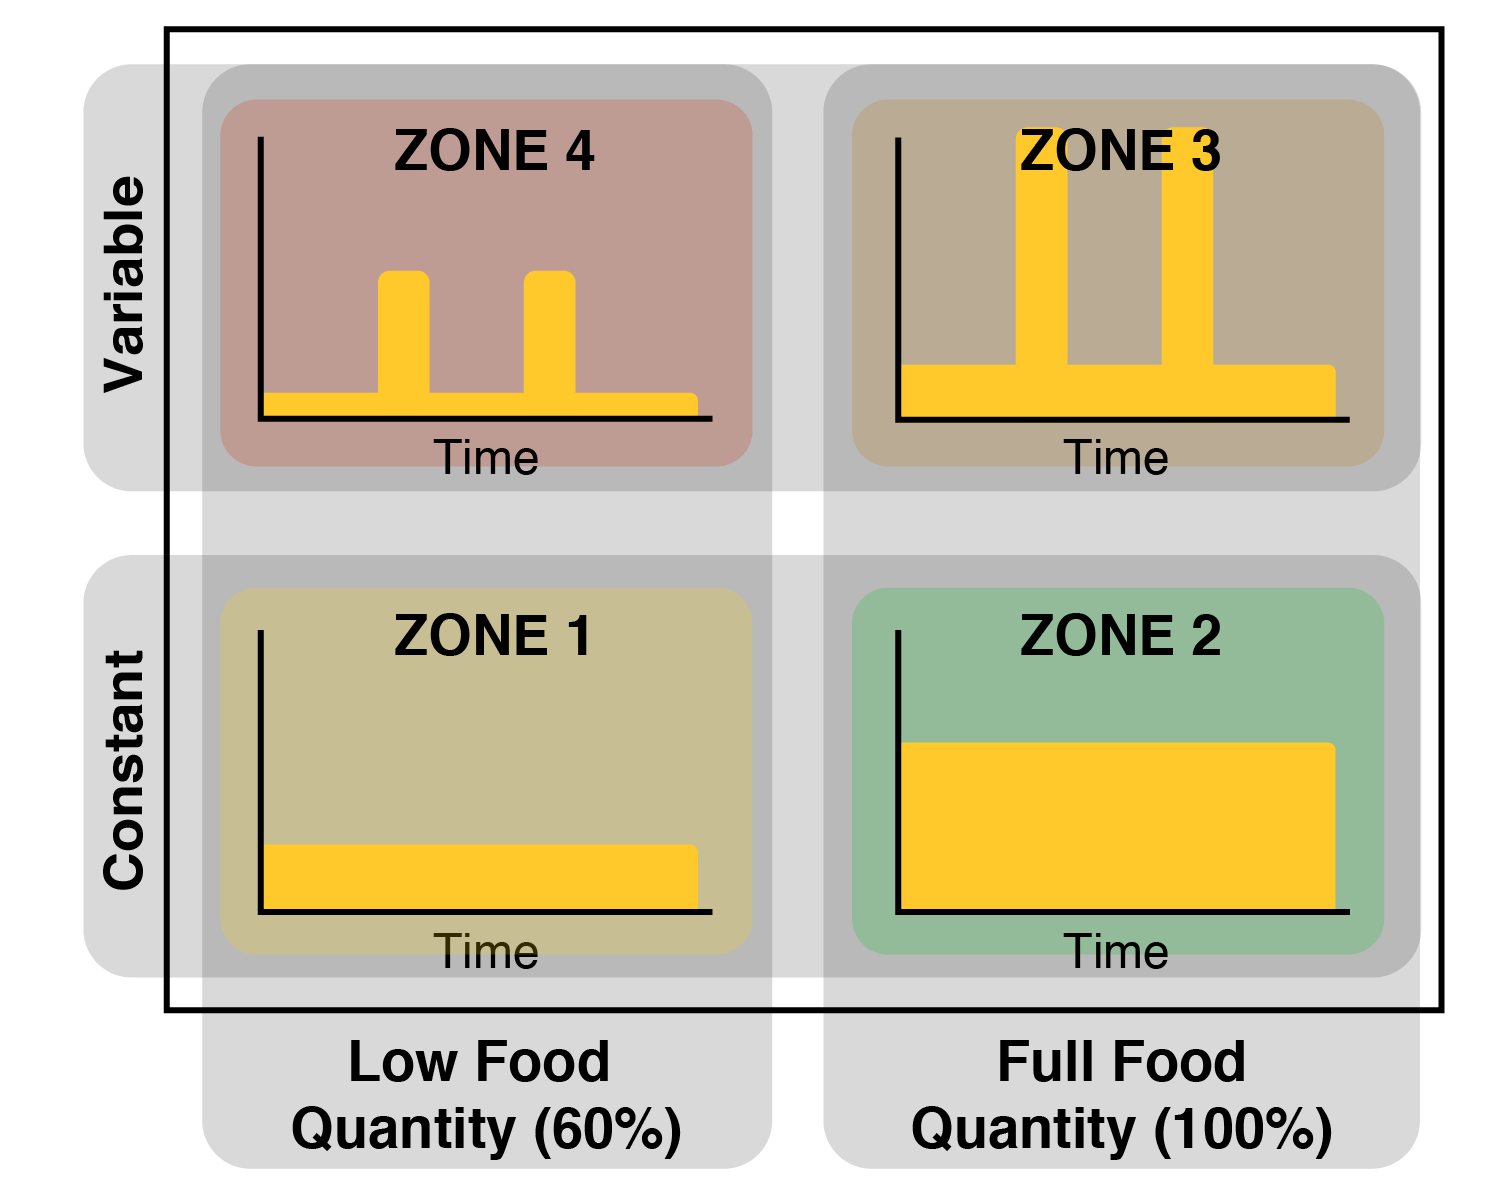
\includegraphics{./fig1_conceptual.png}
\caption{\textbf{Figure 1:} Conceptual depiction of varation in total
resource amount as well as temporal availability. Total resource
abundance increaseses along the x-axis, while temporal variance
increases on the y-axis. The intersecting regions are represented as
``Zones'' of varying food abundance and temporal presentation. We
designed treatments based on these intersections, with diagrams of food
presentation shown in the inset graphs. The area in yellow represents
the amount of food presented to bumble bee microcolonies.}
\end{figure}

\clearpage

\newpage

\begin{figure}
\centering
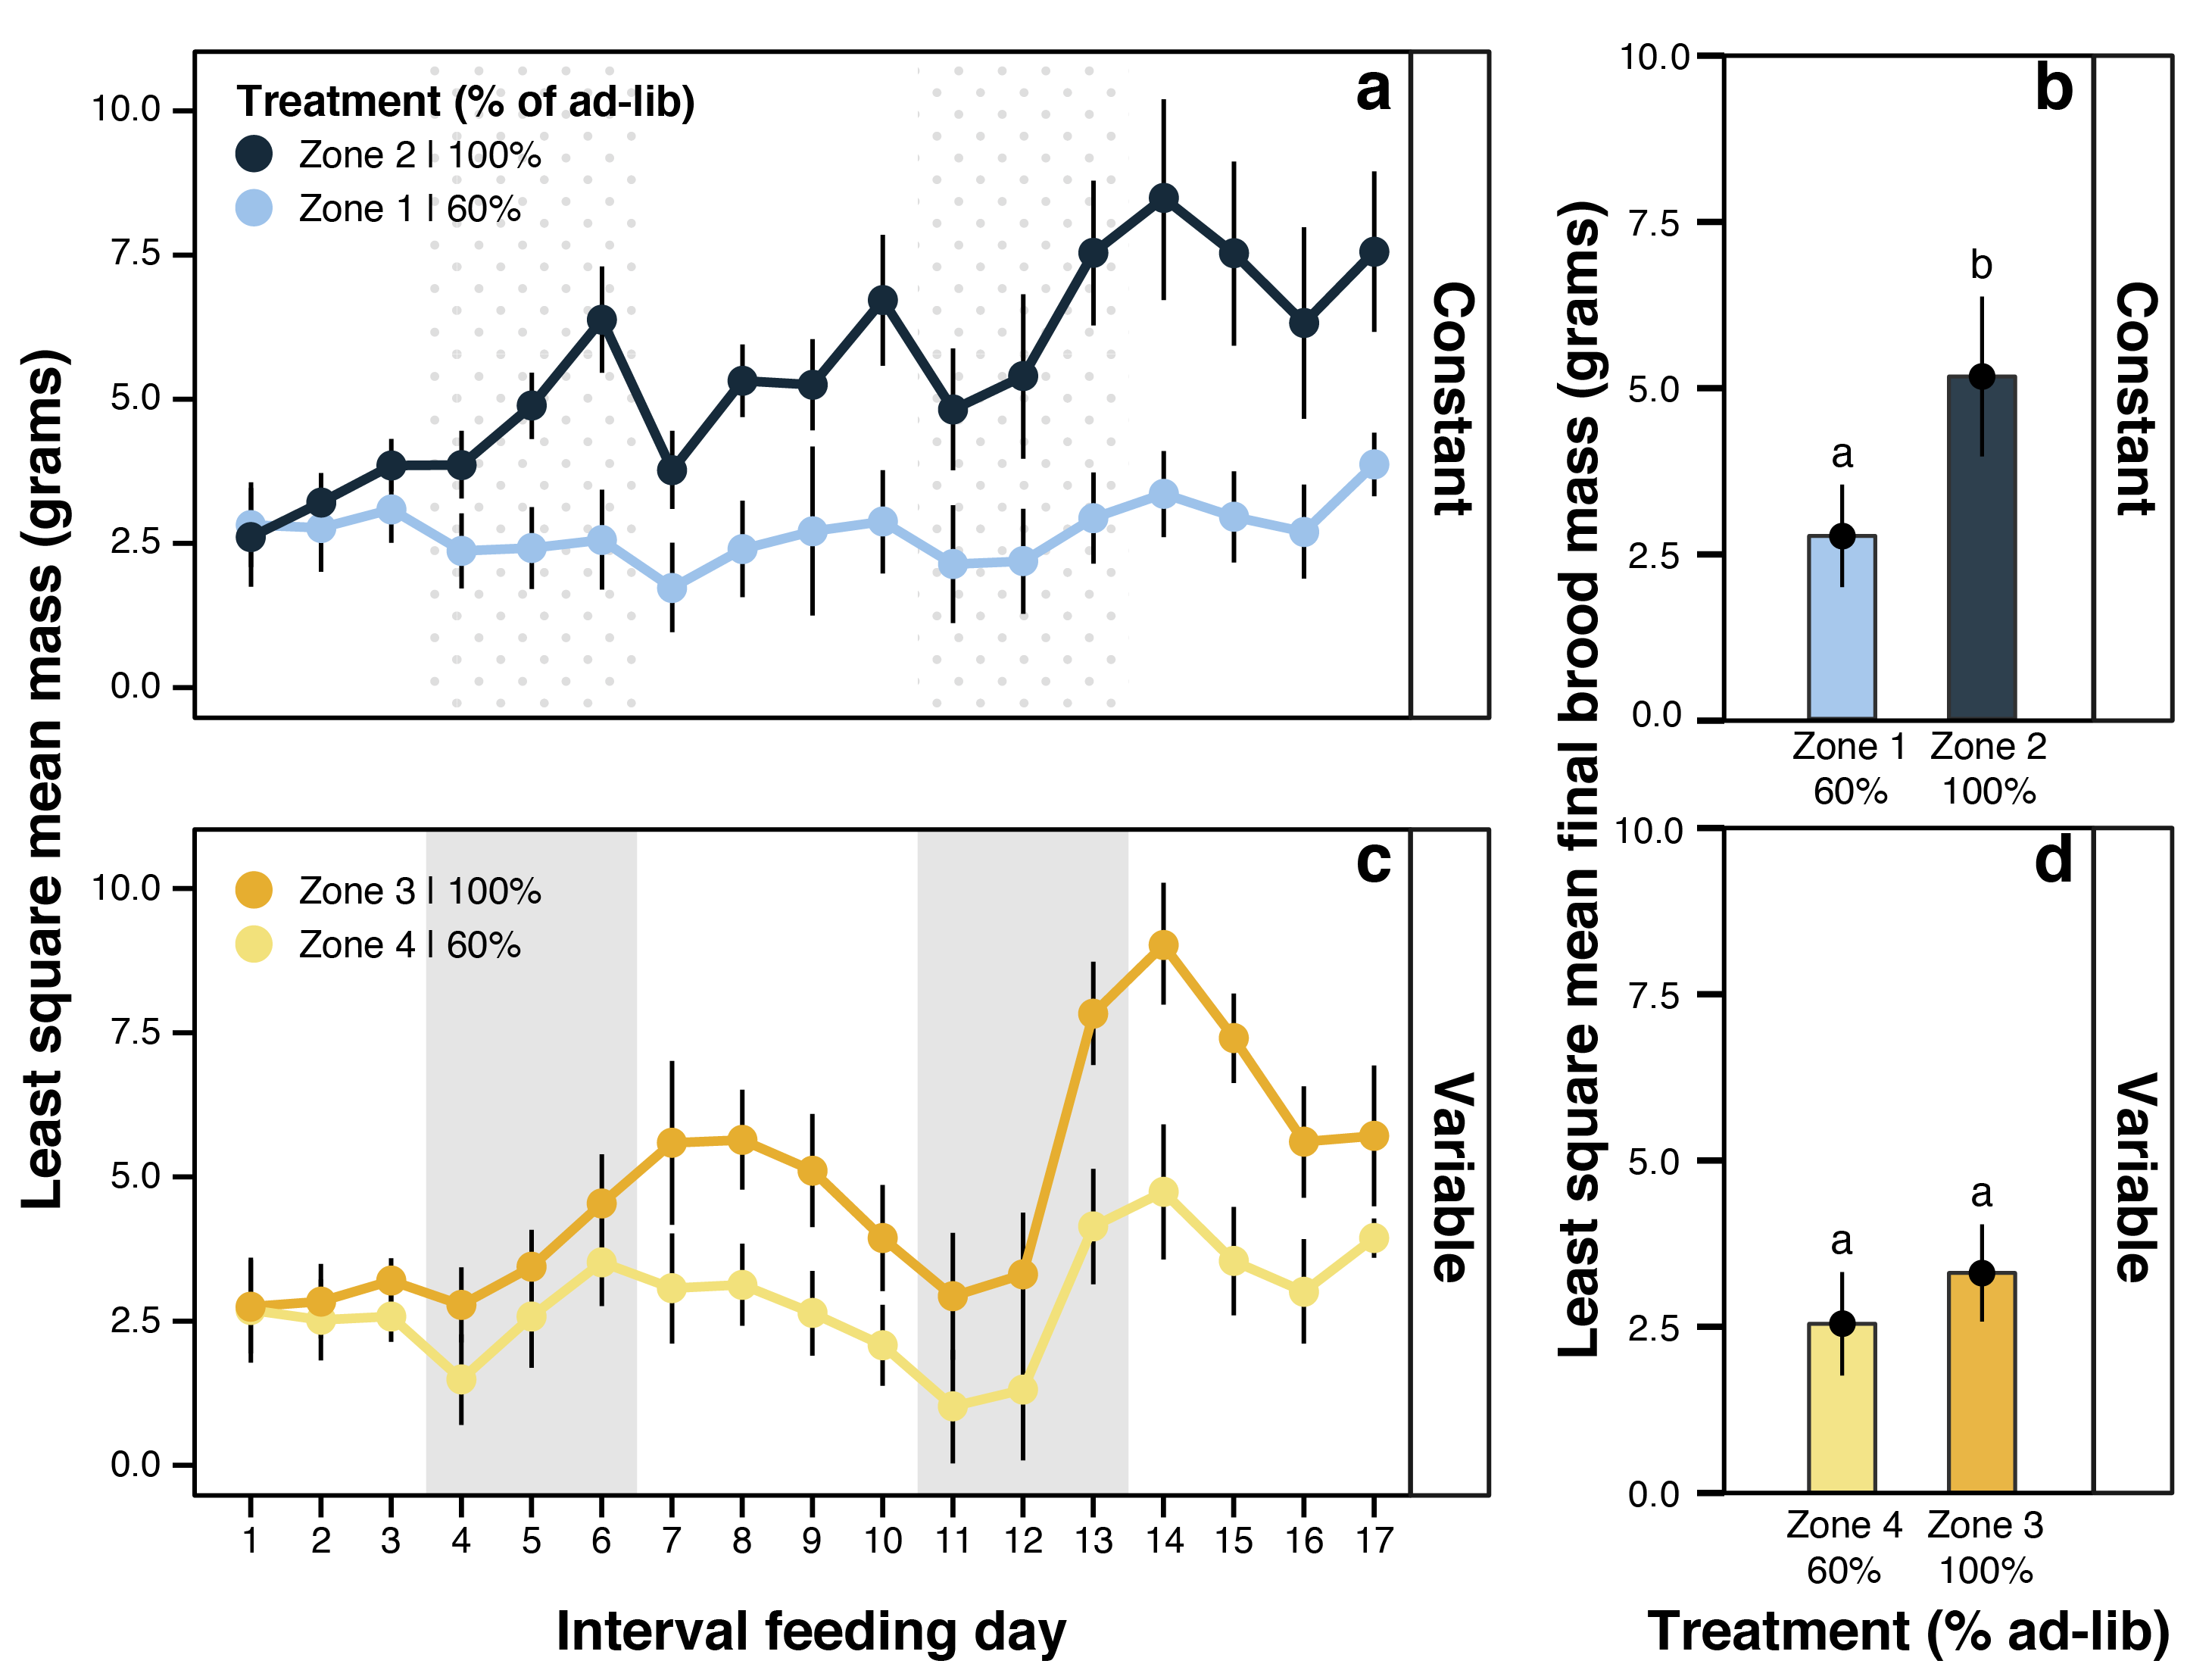
\includegraphics{./fig2_mc_mass.png}
\caption{\textbf{Figure 2:} (a) Least square mean estimated mass
throughout the experiment and (b) Least square mean terminal brood mass.
Letters indicate significant differences both within and across temporal
treatment categories (constant and variable). Error bars represent 95\%
confidence intervals. Difference of 1 interval feeding day is equal to 3
Julian days}
\end{figure}

\clearpage

\newpage

\begin{figure}
\centering
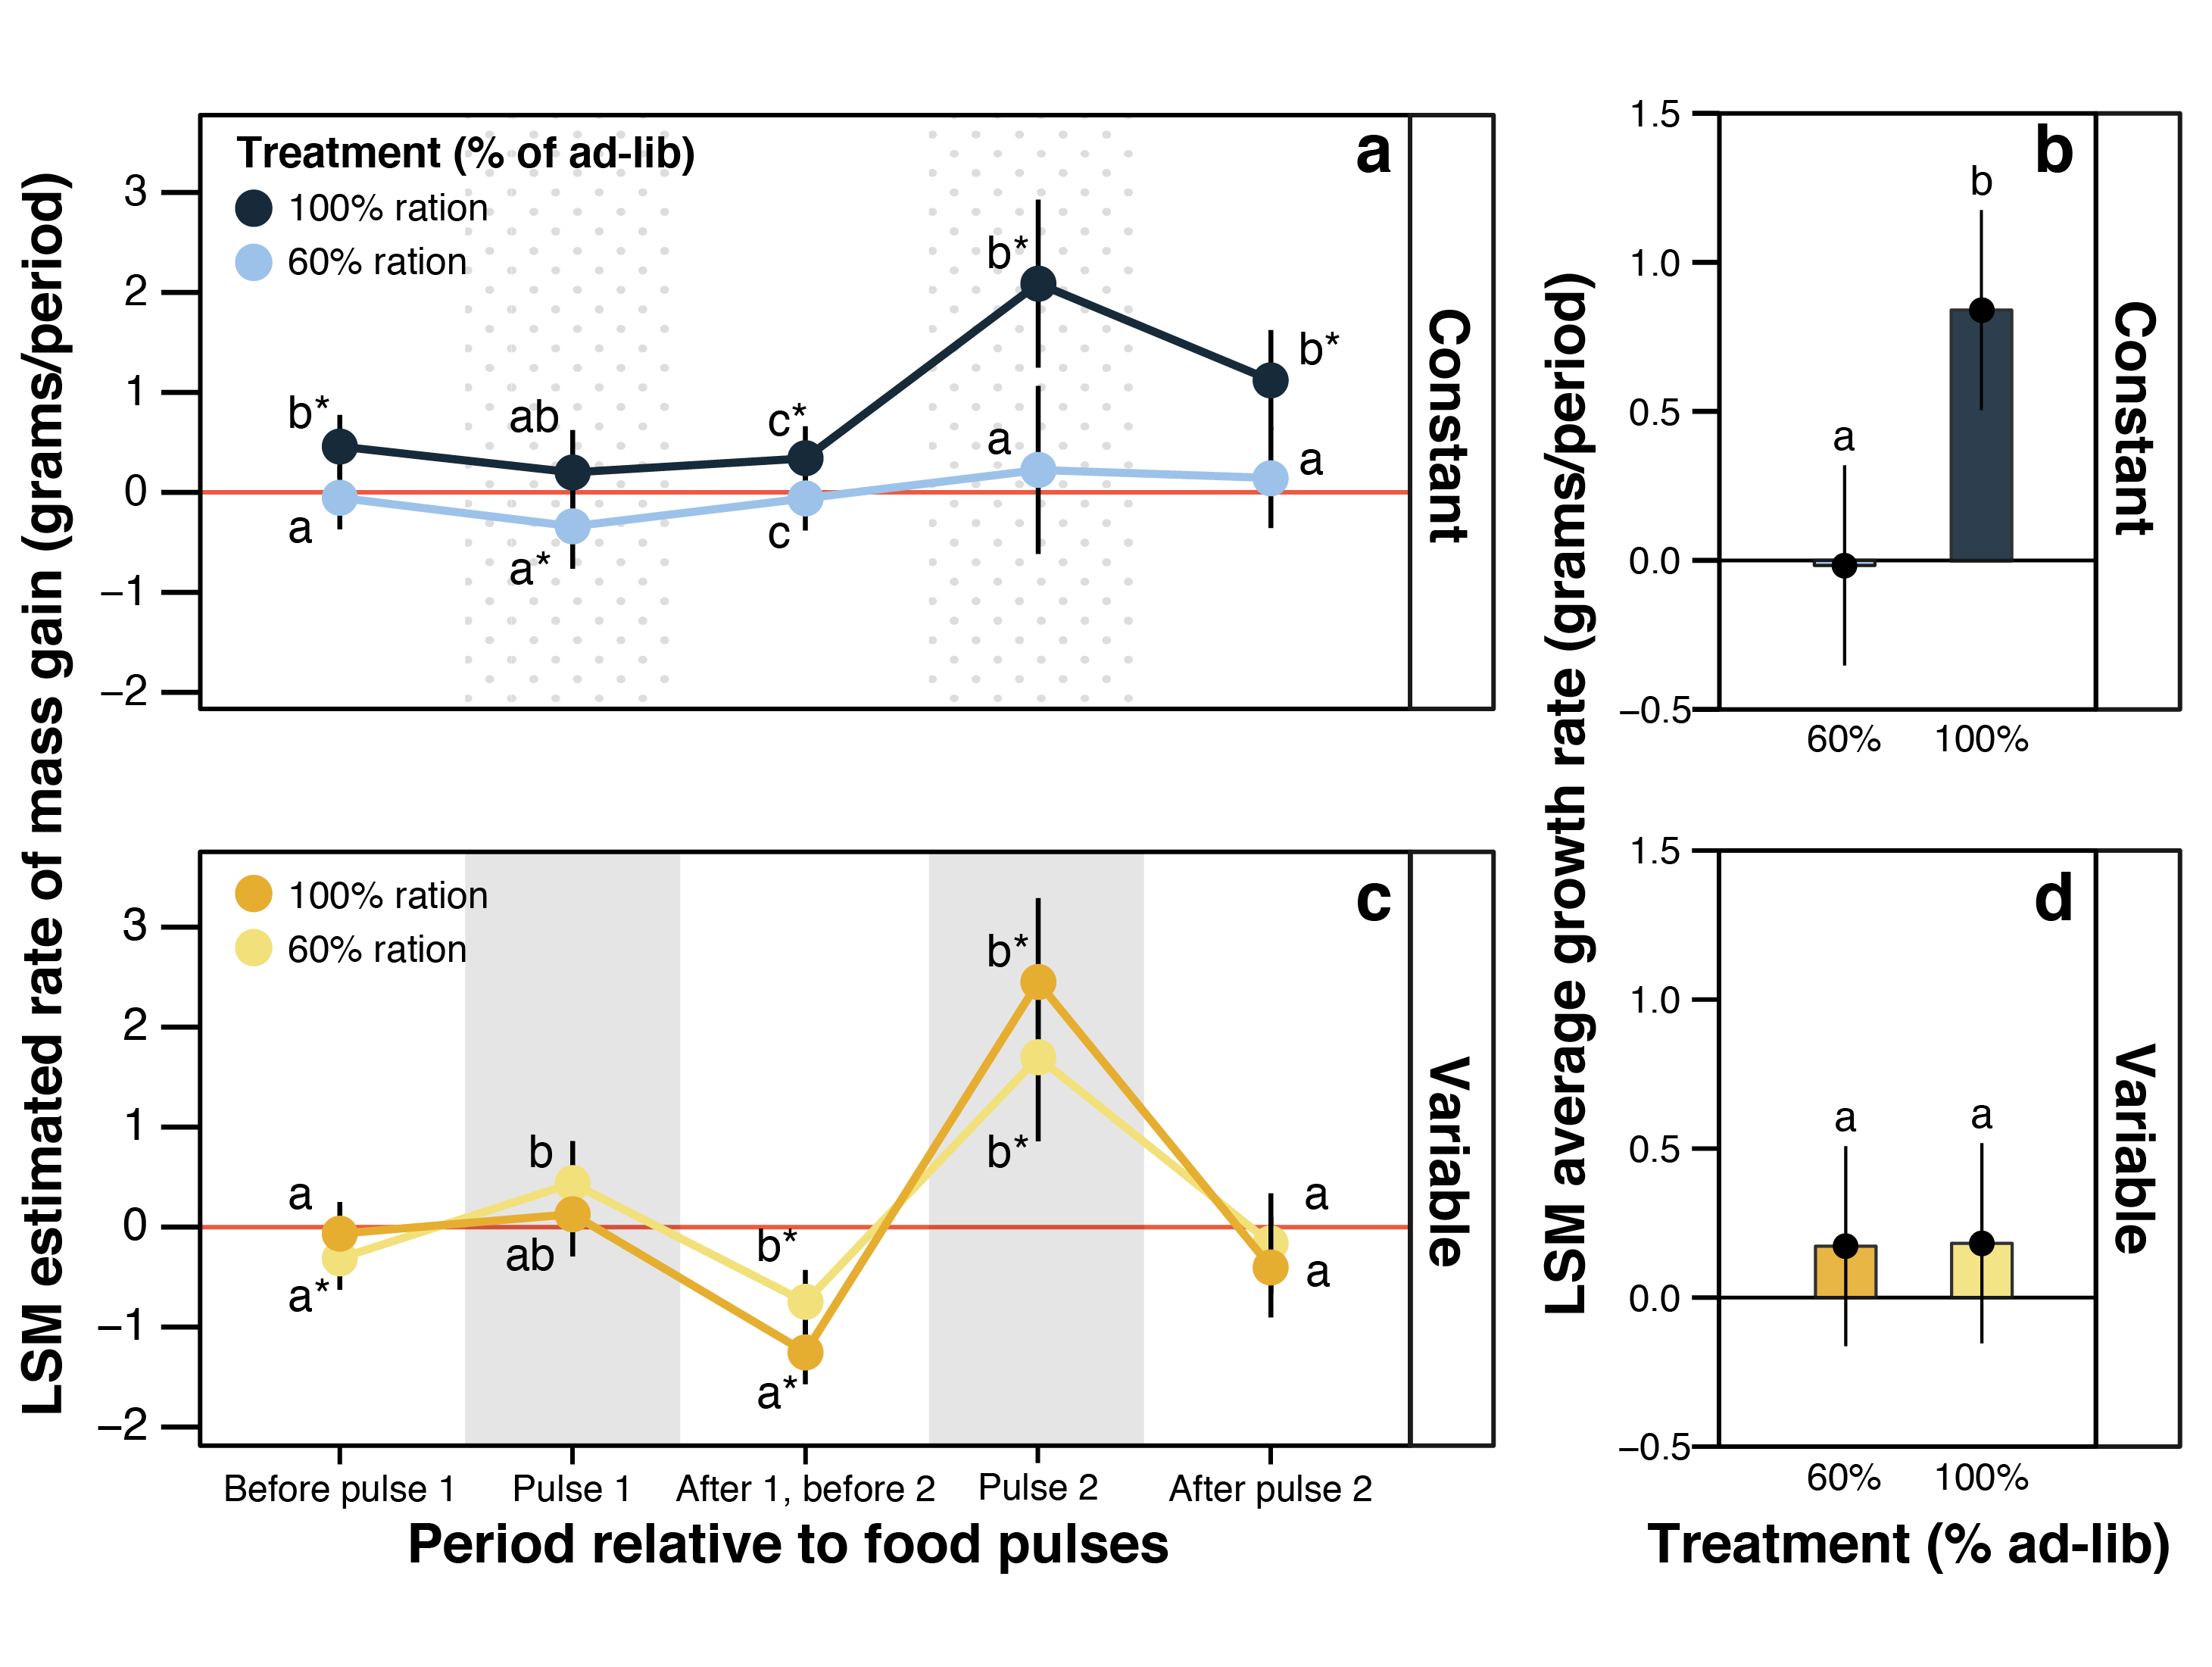
\includegraphics{./fig3_mc_growth.png}
\caption{\textbf{Figure 3:} (a) Least square mean estimated growth rate
by time periods relative to pulses and (b) Least square mean growth
rates by treatment. Letters indicate significant differences both within
and across temporal treatment categories (constant and variable)
\emph{within periods}, while asterisks represent growth estimates
significantly different than 0. Error bars represent 95\% confidence
intervals. Difference of 1 interval feeding day is equal to 3 Julian
days.}
\end{figure}

\clearpage

\newpage

\begin{figure}
\centering
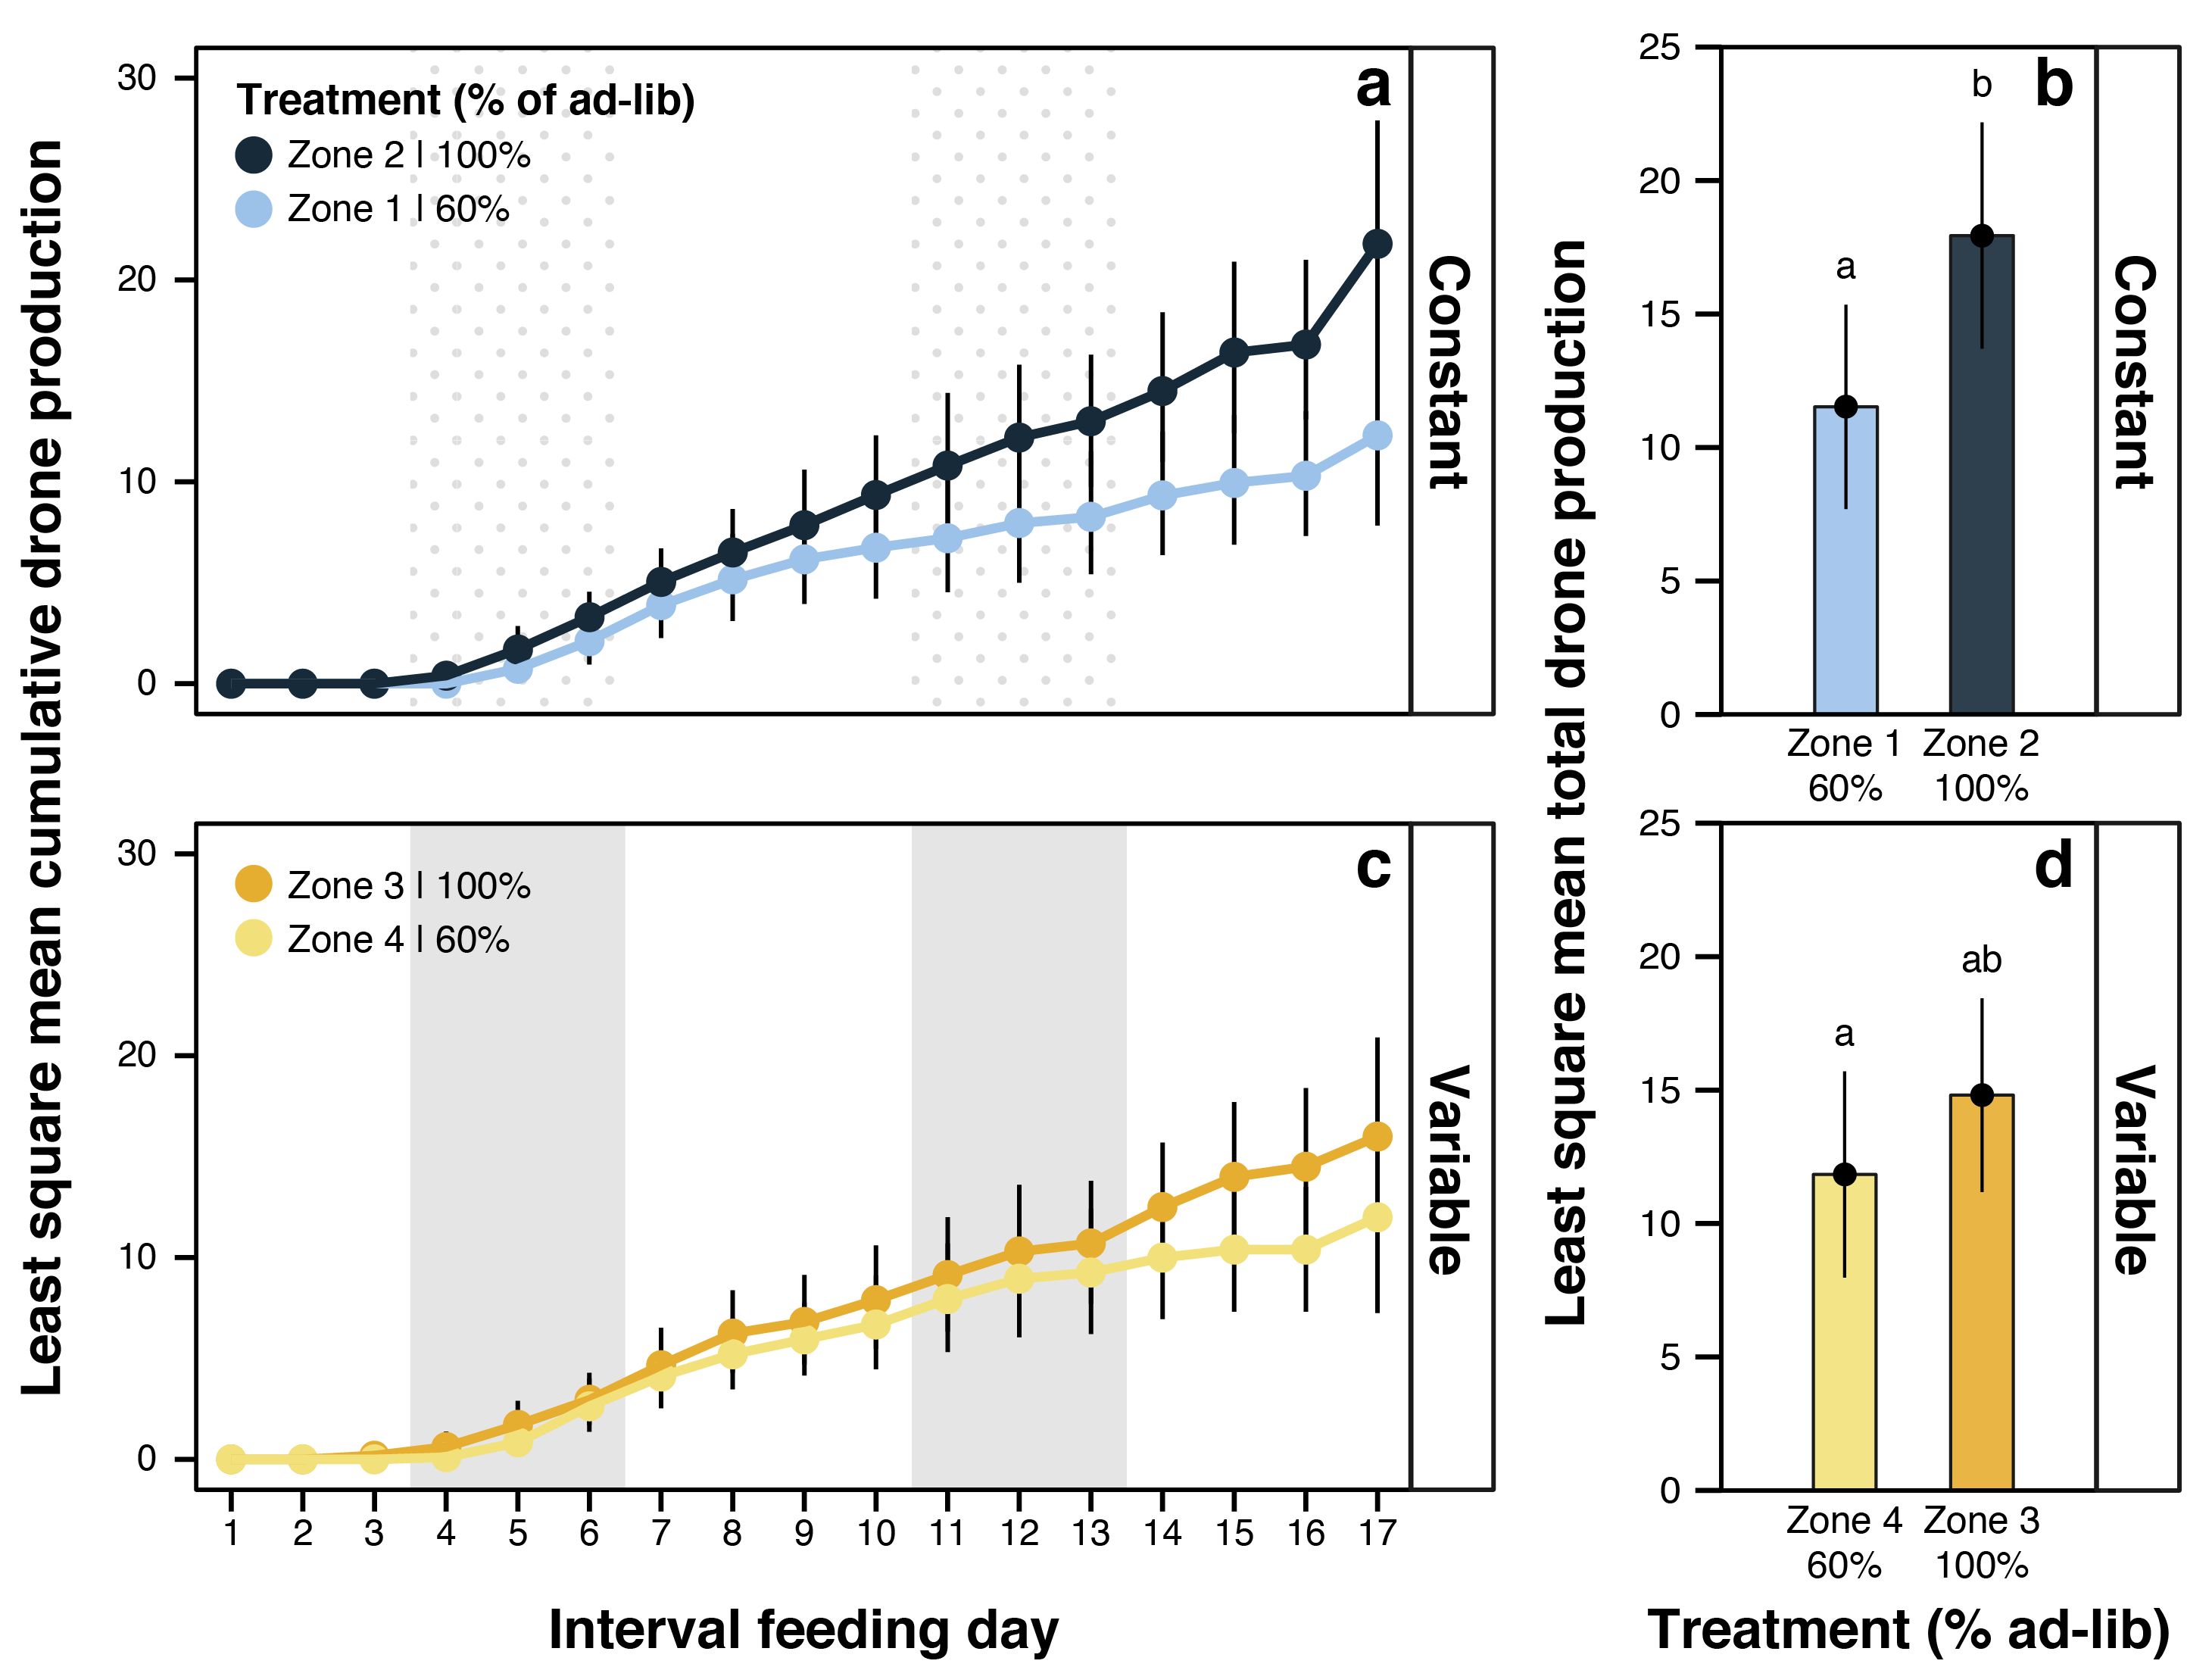
\includegraphics{./fig4_drones.png}
\caption{\textbf{Figure 4:} (a) Least square mean estimated cumulative
drone production and (b) Least square mean total drone production.
Letters indicate significant differences both within and across temporal
treatment categories (constant and variable). Error bars represent 95\%
confidence intervals. Difference of 1 interval feeding day is equal to 3
Julian days.}
\end{figure}

\clearpage

\newpage

\begin{figure}
\centering
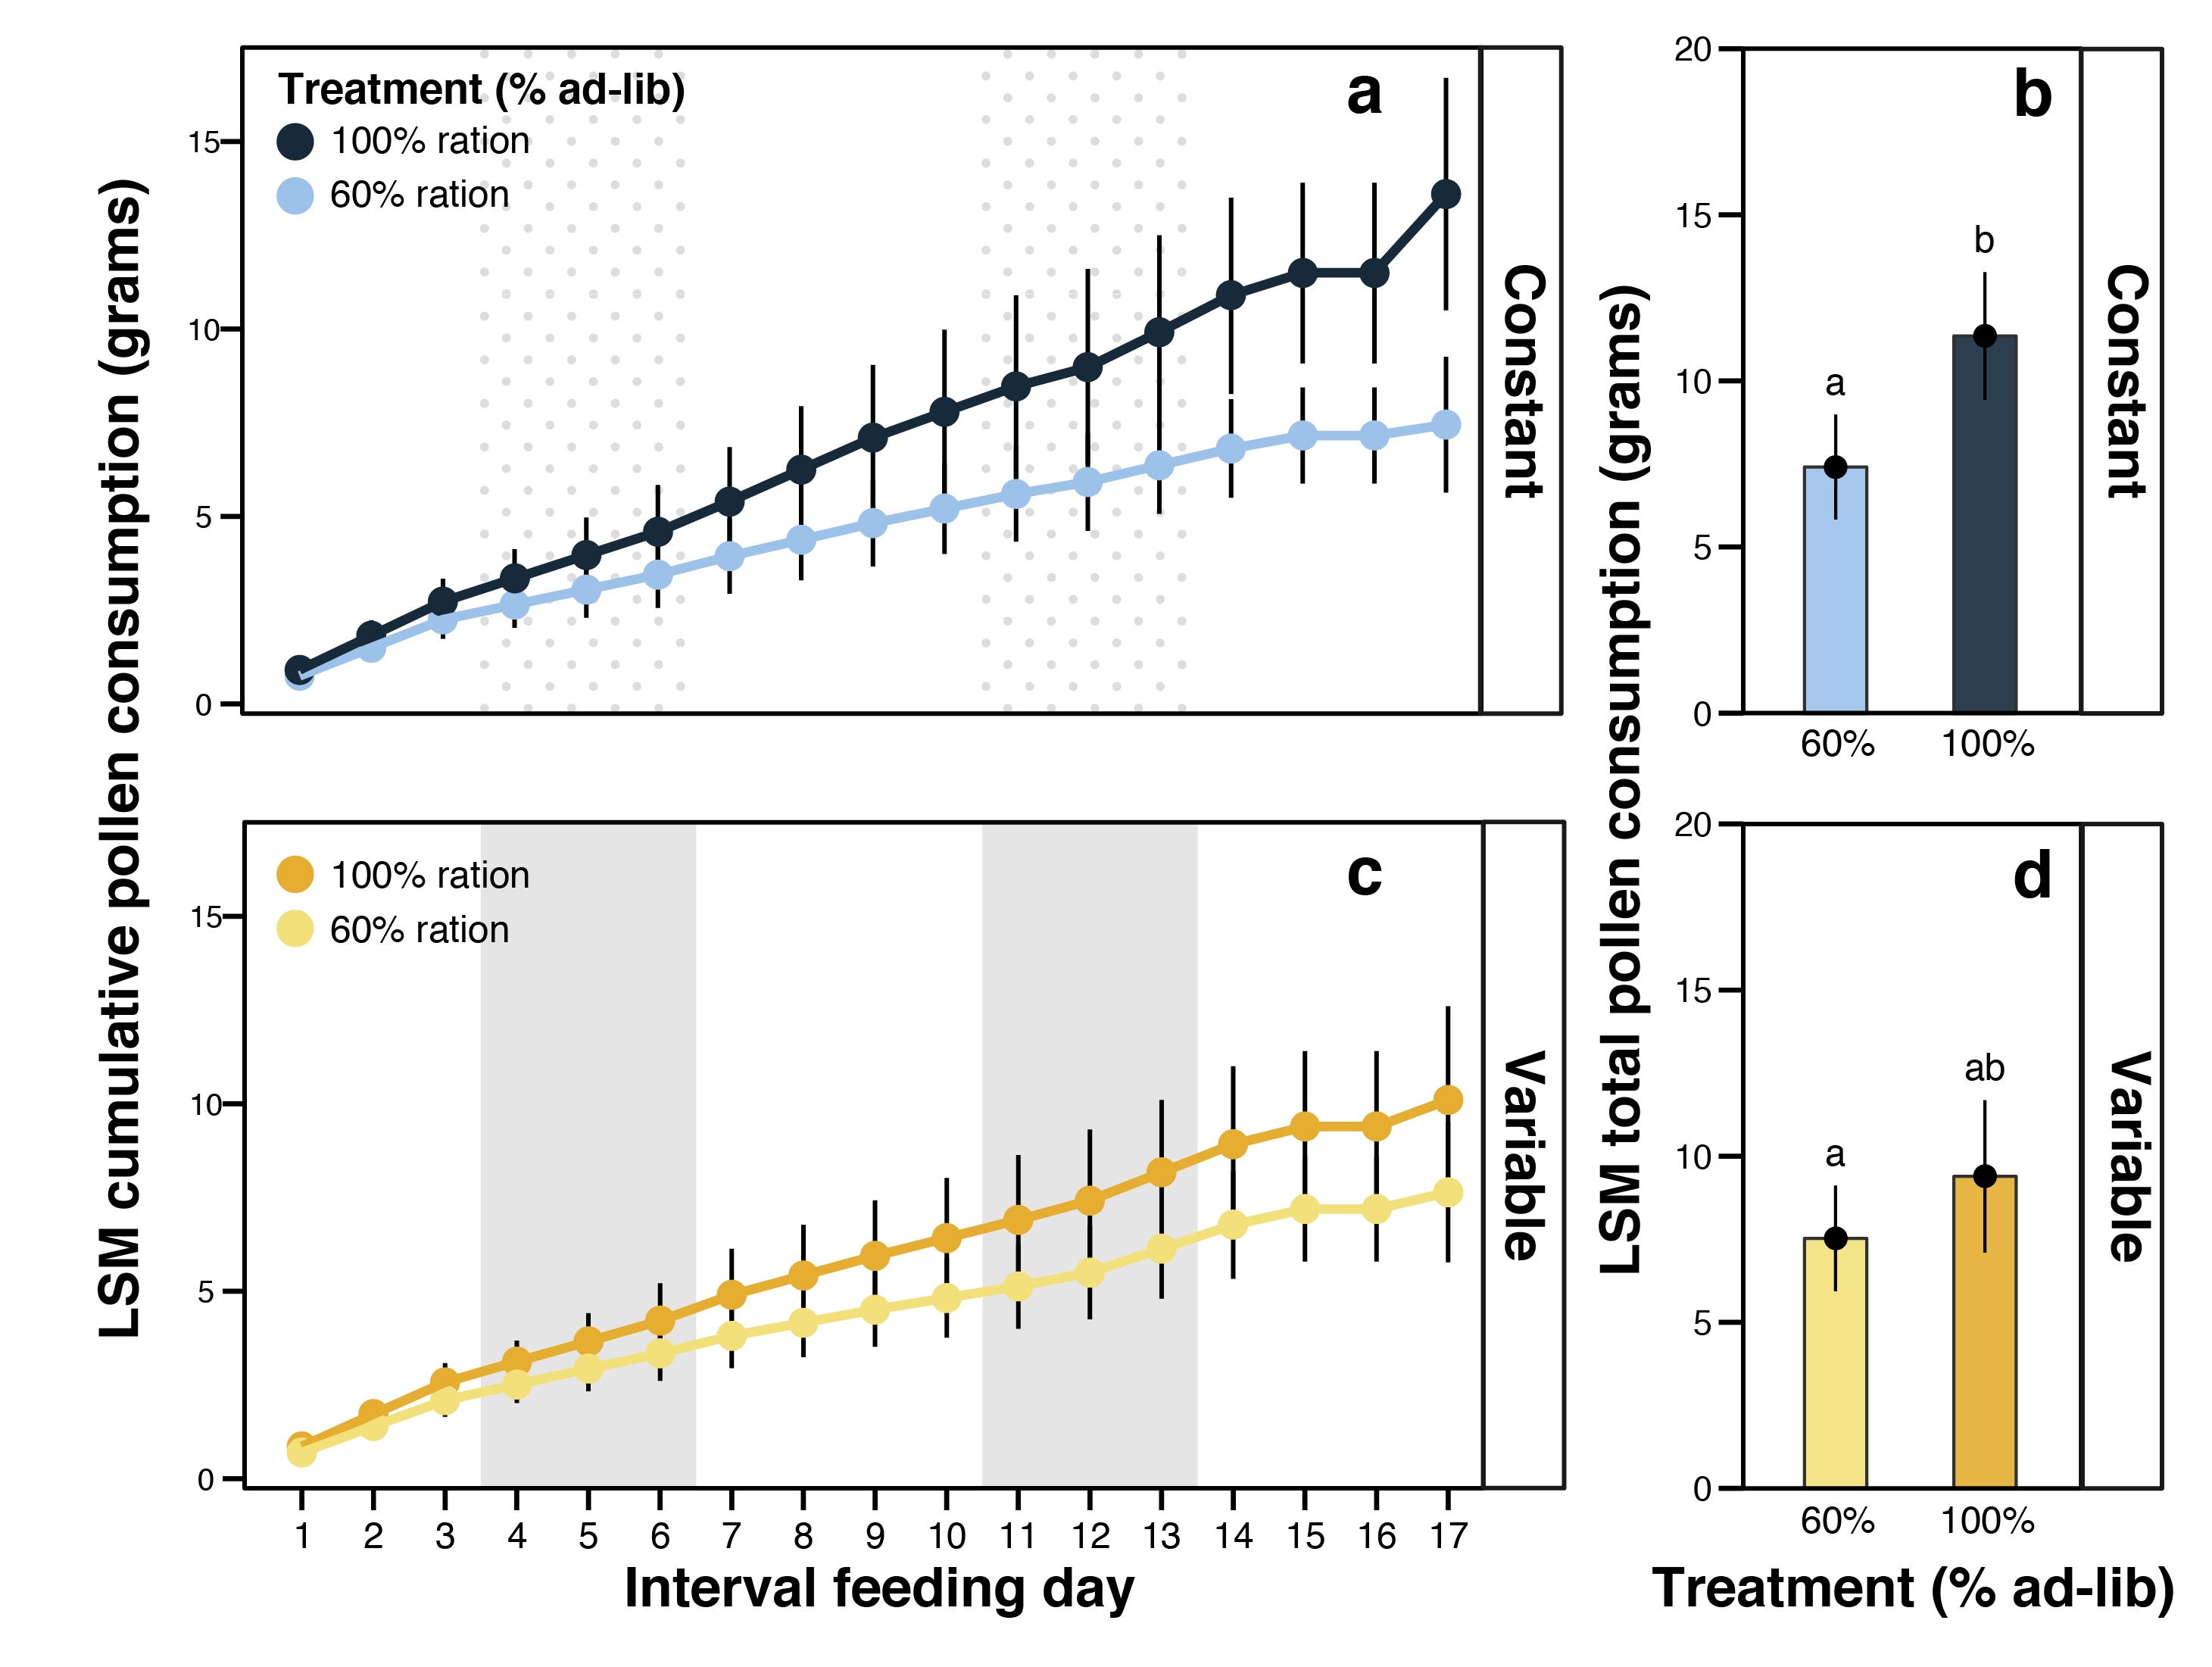
\includegraphics{./supfig1_pollen.png}
\caption{\textbf{Supplemental Figure 1:} (a,c) Least square mean
estimated cumulative pollen consumption (b,d) Least square mean total
pollen consumption by treatment. Letters indicate significant
differences both within and across temporal treatment categories
(constant and variable). Error bars represent 95\% confidence intervals.
Difference of 1 interval feeding day is equal to 3 Julian days.}
\end{figure}

\clearpage

\begin{figure}
\centering
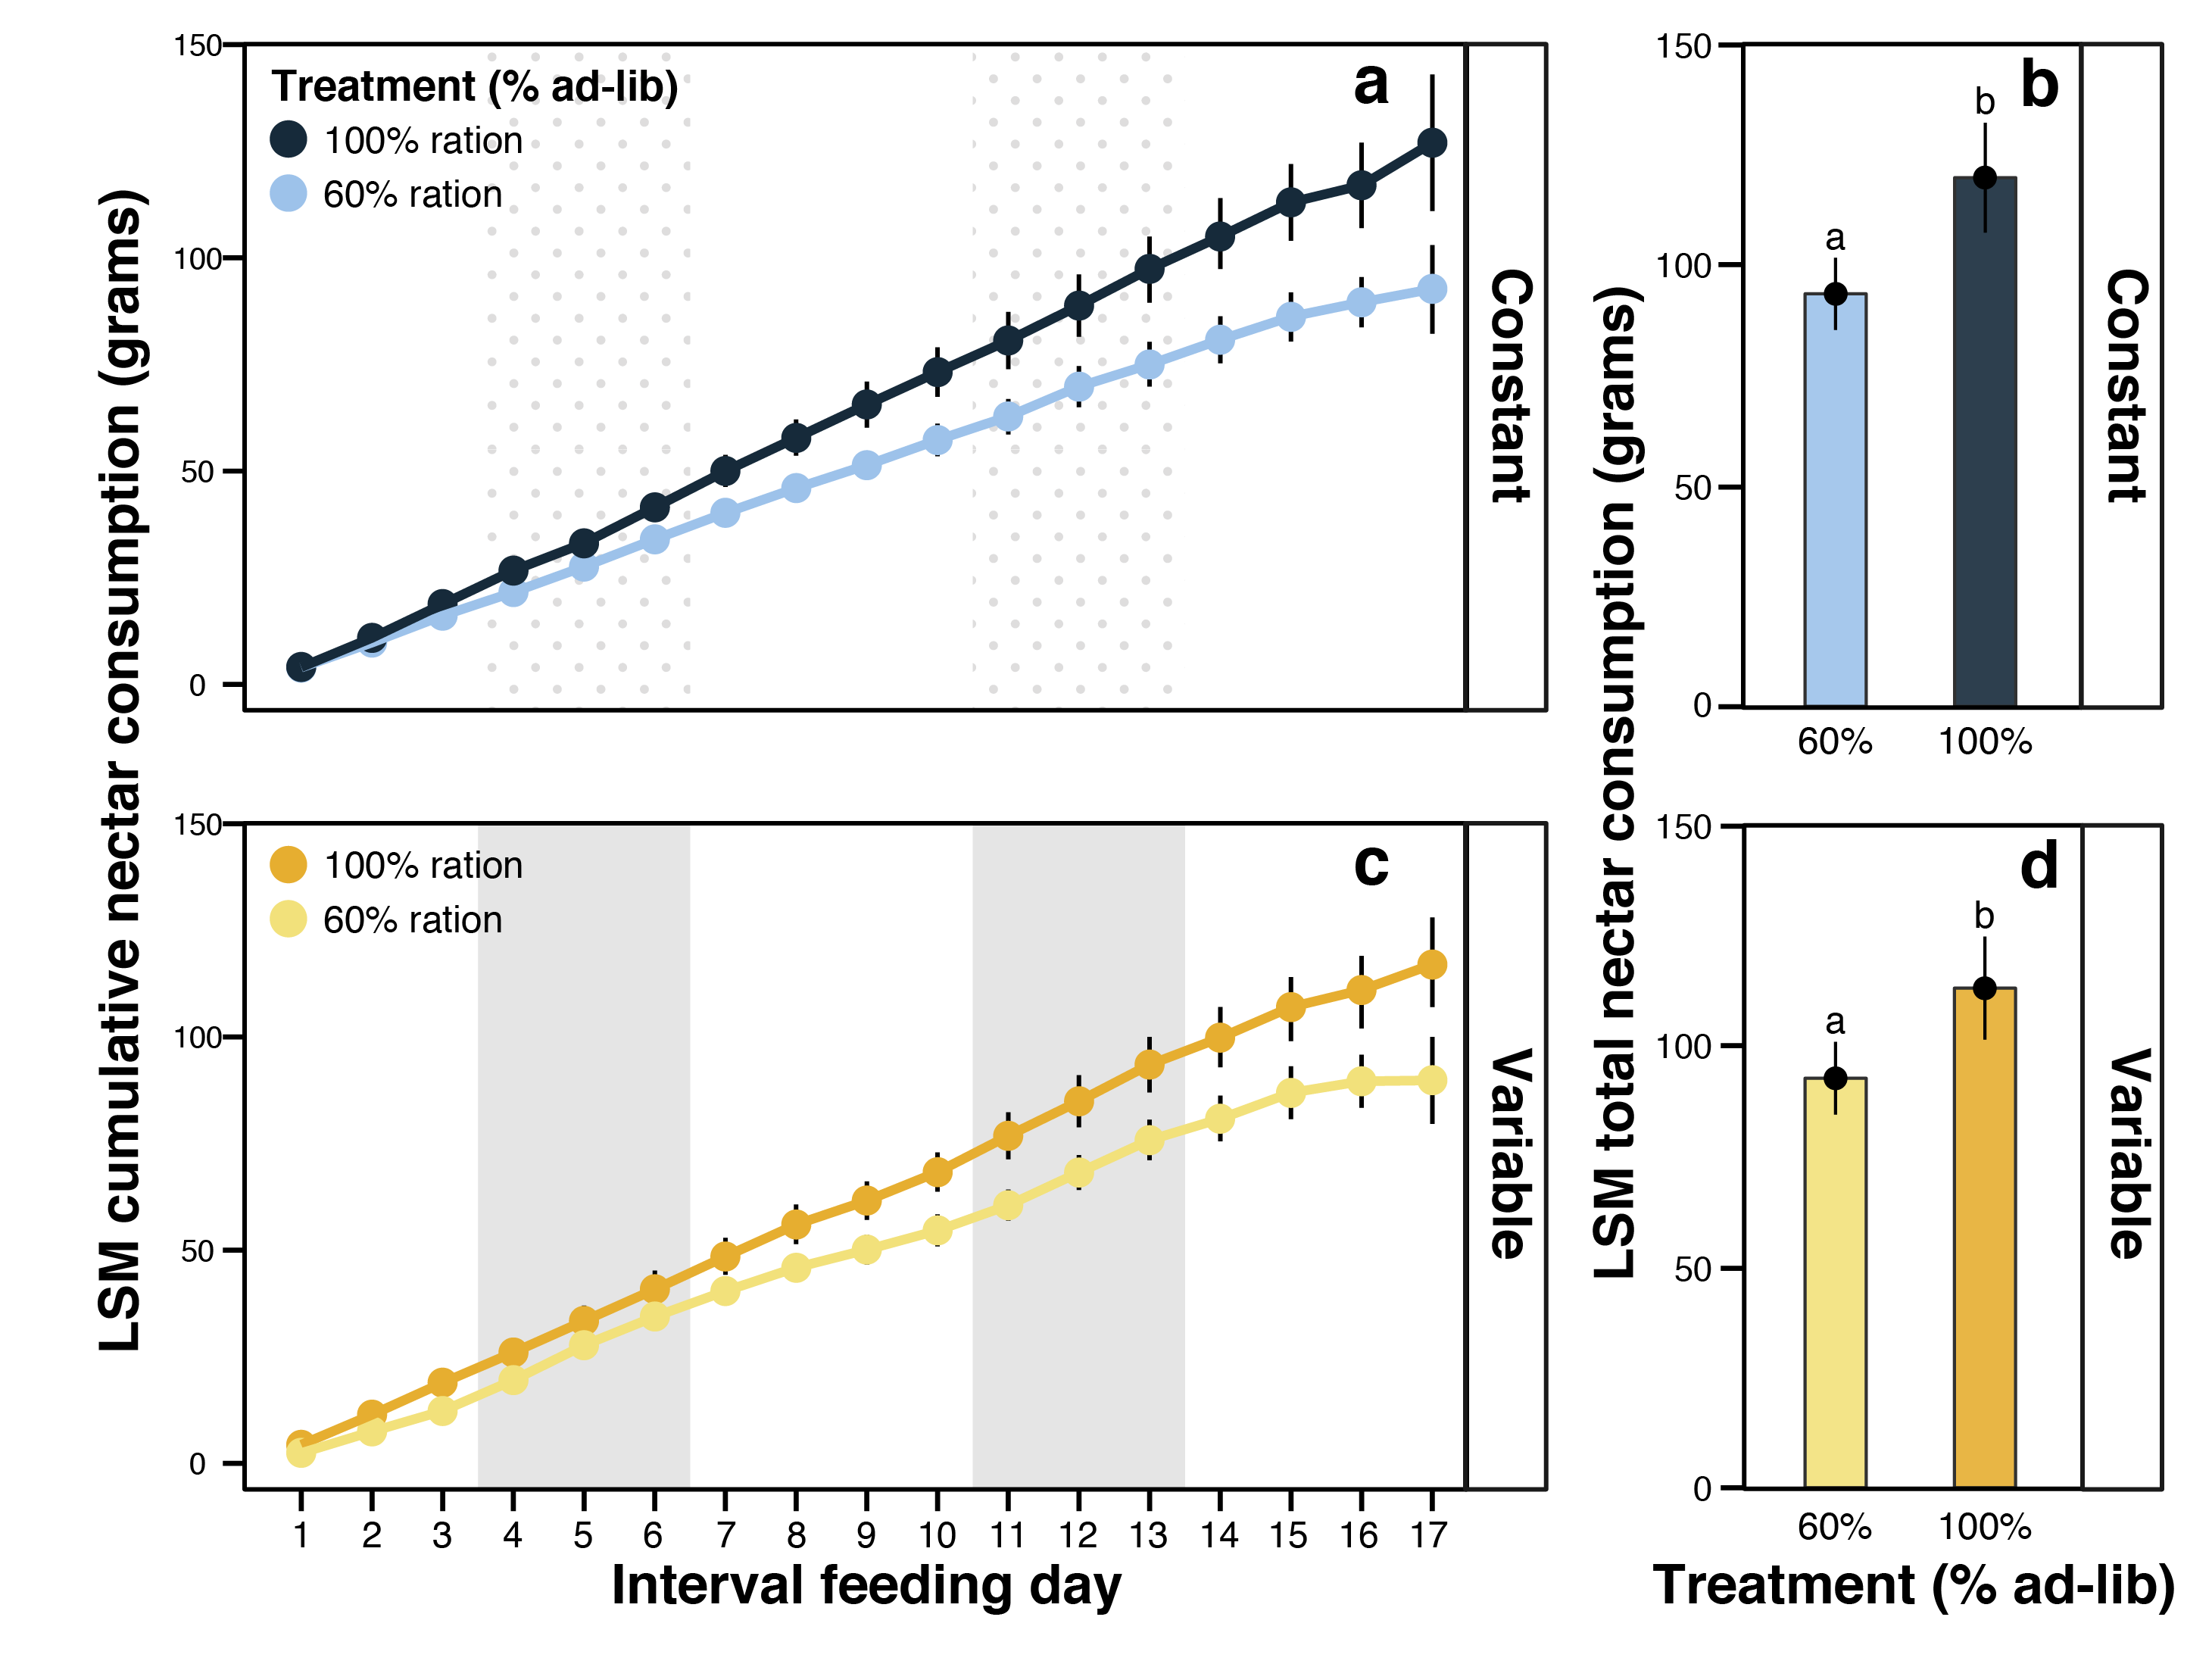
\includegraphics{./supfig2_nectar.png}
\caption{\textbf{Supplemental Figure 2:} (a,c) Least square mean
estimated cumulative nectar consumption (b,d) Least square mean total
nectar consumption by treatment. Letters indicate significant
differences both within and across temporal treatment categories
(constant and variable). Error bars represent 95\% confidence intervals.
Difference of 1 interval feeding day is equal to 3 Julian days.}
\end{figure}

\clearpage

\newpage
\begin{table}[] \centering 
\caption{}{Supplementary Table 1: Mixed model parameter estimates for model with end of experiment microcolony mass as the response variable including 95\% confidence intervals.} 
\begin{tabular}{@{\extracolsep{5pt}}lD{.}{.}{-2} } 
\\[-1.8ex]\hline 
\hline \\[-1.8ex] 
 & \multicolumn{1}{c}{\textit{Response Variable:}} \\ 
\cline{2-2} 
\\[-1.8ex] & \multicolumn{1}{c}{Colony Mass} \\ 
\\[-1.8ex] & \multicolumn{1}{c}{\textit{linear}} \\ 
 & \multicolumn{1}{c}{\textit{mixed effects}} \\ 
\hline \\[-1.8ex] 
 Constant & 5.94^{***}$ $(5.04$, $6.85) \\ 
  trt\_pulse1 & 1.59^{**}$ $(0.69$, $2.49) \\ 
  trt\_total1 & 1.21^{*}$ $(0.30$, $2.11) \\ 
  rep & -1.26^{***}$ $(-1.67$, $-0.85) \\ 
  trt\_pulse1:trt\_total1 & 1.18^{*}$ $(0.28$, $2.08) \\ 
  trt\_pulse1:rep & -0.54^{*}$ $(-0.95$, $-0.13) \\ 
  trt\_total1:rep & -0.20$ $(-0.61$, $0.21) \\ 
  trt\_pulse1:trt\_total1:rep & -0.38$ $(-0.79$, $0.03) \\ 
 \hline \\[-1.8ex] 
Observations & \multicolumn{1}{c}{80} \\ 
Log Likelihood & \multicolumn{1}{c}{-147.64} \\ 
Akaike Inf. Crit. & \multicolumn{1}{c}{315.28} \\ 
Bayesian Inf. Crit. & \multicolumn{1}{c}{338.05} \\ 
\hline 
\hline \\[-1.8ex] 
\textit{Note:}  & \multicolumn{1}{r}{$^{*}$p$<$0.05; $^{**}$p$<$0.01; $^{***}$p$<$0.001} \\ 
\end{tabular} 
\end{table} 
\clearpage

\newpage
\begin{table}[] \centering 
\caption{}{Supplementary Table 2: Mixed model parameter estimates for model with rate of mass gain as the response variable including 95\% confidence intervals.} 
  \label{suptab2} 
\begin{tabular}{@{\extracolsep{5pt}}lD{.}{.}{-2} } 
\\[-1.8ex]\hline 
\hline \\[-1.8ex] 
 & \multicolumn{1}{c}{\textit{Response Variable:}} \\ 
\cline{2-2} 
\\[-1.8ex] & \multicolumn{1}{c}{Rate of Mass Gain} \\ 
\\[-1.8ex] & \multicolumn{1}{c}{\textit{linear}} \\ 
 & \multicolumn{1}{c}{\textit{mixed effects}} \\ 
\hline \\[-1.8ex] 
 Constant & 0.21^{***}$ $(0.10$, $0.32) \\ 
  trt\_pulse1 & 0.07$ $(-0.04$, $0.18) \\ 
  trt\_total1 & 0.13^{*}$ $(0.02$, $0.24) \\ 
  pulse\_cat1 & -0.67^{***}$ $(-0.89$, $-0.45) \\ 
  pulse\_cat2 & -0.40^{***}$ $(-0.62$, $-0.18) \\ 
  pulse\_cat3 & -0.23^{*}$ $(-0.45$, $-0.01) \\ 
  pulse\_cat4 & -0.14$ $(-0.36$, $0.08) \\ 
  trt\_pulse1:trt\_total1 & 0.20^{**}$ $(0.09$, $0.31) \\ 
 \hline \\[-1.8ex] 
Observations & \multicolumn{1}{c}{140} \\ 
Log Likelihood & \multicolumn{1}{c}{-150.53} \\ 
Akaike Inf. Crit. & \multicolumn{1}{c}{321.06} \\ 
Bayesian Inf. Crit. & \multicolumn{1}{c}{349.89} \\ 
\hline 
\hline \\[-1.8ex] 
\textit{Note:}  & \multicolumn{1}{r}{$^{*}$p$<$0.05; $^{**}$p$<$0.01; $^{***}$p$<$0.001} \\ 
\end{tabular} 
\end{table} 
\clearpage

\newpage
\begin{table}[] \centering 
\caption{}{Supplementary Table 3: Mixed model parameter estimates for repeated measures model with mass as the response variable including 95\% confidence intervals.} 
  \label{} 
\begin{tabular}{@{\extracolsep{5pt}}lD{.}{.}{-2} } 
\\[-1.8ex]\hline 
\hline \\[-1.8ex] 
 & \multicolumn{1}{c}{\textit{Response Variable:}} \\ 
\cline{2-2} 
\\[-1.8ex] & \multicolumn{1}{c}{Mass Gain (Temporal trends)} \\ 
\\[-1.8ex] & \multicolumn{1}{c}{\textit{linear}} \\ 
 & \multicolumn{1}{c}{\textit{mixed effects}} \\ 
\hline \\[-1.8ex] 
 Constant & -793.66^{***}$ $(-982.99$, $-604.33) \\ 
  trt\_total1 & 1.15^{***}$ $(0.94$, $1.36) \\ 
  trt\_pulse1 & 0.13$ $(-0.08$, $0.34) \\ 
  rep1 & 4.88^{***}$ $(3.66$, $6.09) \\ 
  rep2 & 0.04$ $(-0.33$, $0.41) \\ 
  date & 0.04^{***}$ $(0.03$, $0.06) \\ 
  trt\_total1:trt\_pulse1 & 0.19$ $(-0.02$, $0.40) \\ 
  trt\_total1:rep1 & 0.21$ $(-0.09$, $0.51) \\ 
  trt\_total1:rep2 & -0.07$ $(-0.37$, $0.23) \\ 
  trt\_pulse1:rep1 & 0.44^{**}$ $(0.14$, $0.74) \\ 
  trt\_pulse1:rep2 & -0.27$ $(-0.57$, $0.03) \\ 
  trt\_total1:trt\_pulse1:rep1 & 0.35^{*}$ $(0.06$, $0.65) \\ 
  trt\_total1:trt\_pulse1:rep2 & -0.25$ $(-0.55$, $0.05) \\ 
 \hline \\[-1.8ex] 
Observations & \multicolumn{1}{c}{1,315} \\ 
Log Likelihood & \multicolumn{1}{c}{-2,589.40} \\ 
Akaike Inf. Crit. & \multicolumn{1}{c}{5,228.81} \\ 
Bayesian Inf. Crit. & \multicolumn{1}{c}{5,358.10} \\ 
\hline 
\hline \\[-1.8ex] 
\textit{Note:}  & \multicolumn{1}{r}{$^{*}$p$<$0.05; $^{**}$p$<$0.01; $^{***}$p$<$0.001} \\ 
\end{tabular} 
\end{table} 
\clearpage

\newpage
\begin{table}[] \centering 
\caption{}{Supplementary Table 4: Mixed model parameter estimates for model with cumulative drone production as the response variable including 95\% confidence intervals.} 
  \label{} 
\begin{tabular}{@{\extracolsep{5pt}}lD{.}{.}{-2} } 
\\[-1.8ex]\hline 
\hline \\[-1.8ex] 
 & \multicolumn{1}{c}{\textit{Response Variable:}} \\ 
\cline{2-2} 
\\[-1.8ex] & \multicolumn{1}{c}{Drone Production} \\ 
\\[-1.8ex] & \multicolumn{1}{c}{\textit{linear}} \\ 
 & \multicolumn{1}{c}{\textit{mixed effects}} \\ 
\hline \\[-1.8ex] 
 Constant & 29.02^{***}$ $(24.92$, $33.12) \\ 
  trt\_pulse1 & 2.62$ $(-1.48$, $6.72) \\ 
  trt\_total1 & 4.53^{*}$ $(0.43$, $8.63) \\ 
  rep & -7.43^{***}$ $(-9.29$, $-5.57) \\ 
  trt\_pulse1:trt\_total1 & 2.70$ $(-1.40$, $6.80) \\ 
  trt\_pulse1:rep & -0.85$ $(-2.70$, $1.01) \\ 
  trt\_total1:rep & -1.05$ $(-2.91$, $0.80) \\ 
  trt\_pulse1:trt\_total1:rep & -0.92$ $(-2.78$, $0.94) \\ 
 \hline \\[-1.8ex] 
Observations & \multicolumn{1}{c}{77} \\ 
Log Likelihood & \multicolumn{1}{c}{-245.15} \\ 
Akaike Inf. Crit. & \multicolumn{1}{c}{510.30} \\ 
Bayesian Inf. Crit. & \multicolumn{1}{c}{532.64} \\ 
\hline 
\hline \\[-1.8ex] 
\textit{Note:}  & \multicolumn{1}{r}{$^{*}$p$<$0.05; $^{**}$p$<$0.01; $^{***}$p$<$0.001} \\ 
\end{tabular} 
\end{table}
\clearpage

\newpage
\begin{table}[] \centering 
\caption{}{Supplementary Table 5: Mixed model parameter estimates for model with time to first drone as the response variable including 95\% confidence intervals.} 
  \label{} 
\begin{tabular}{@{\extracolsep{5pt}}lD{.}{.}{-2} } 
\\[-1.8ex]\hline 
\hline \\[-1.8ex] 
 & \multicolumn{1}{c}{\textit{Response Variable:}} \\ 
\cline{2-2} 
\\[-1.8ex] & \multicolumn{1}{c}{Time to First Drone} \\ 
\\[-1.8ex] & \multicolumn{1}{c}{\textit{linear}} \\ 
 & \multicolumn{1}{c}{\textit{mixed effects}} \\ 
\hline \\[-1.8ex] 
 Constant & 17.24^{***}$ $(16.12$, $18.35) \\ 
  trt\_total1 & -0.50$ $(-1.62$, $0.61) \\ 
  trt\_pulse1 & 0.82$ $(-0.29$, $1.94) \\ 
  rep1 & -4.18^{***}$ $(-5.47$, $-2.88) \\ 
  rep2 & -2.23^{**}$ $(-3.47$, $-0.98) \\ 
  trt\_total1:trt\_pulse1 & -0.95$ $(-2.07$, $0.17) \\ 
  trt\_total1:rep1 & -0.63$ $(-1.92$, $0.67) \\ 
  trt\_total1:rep2 & 0.06$ $(-1.18$, $1.31) \\ 
  trt\_pulse1:rep1 & 0.19$ $(-1.11$, $1.48) \\ 
  trt\_pulse1:rep2 & -0.55$ $(-1.80$, $0.70) \\ 
  trt\_total1:trt\_pulse1:rep1 & 1.15$ $(-0.15$, $2.45) \\ 
  trt\_total1:trt\_pulse1:rep2 & 0.24$ $(-1.01$, $1.49) \\ 
 \hline \\[-1.8ex] 
Observations & \multicolumn{1}{c}{75} \\ 
Log Likelihood & \multicolumn{1}{c}{-204.21} \\ 
Akaike Inf. Crit. & \multicolumn{1}{c}{436.42} \\ 
Bayesian Inf. Crit. & \multicolumn{1}{c}{466.42} \\ 
\hline 
\hline \\[-1.8ex] 
\textit{Note:}  & \multicolumn{1}{r}{$^{*}$p$<$0.05; $^{**}$p$<$0.01; $^{***}$p$<$0.001} \\ 
\end{tabular} 
\end{table} 
\clearpage

\newpage
\begin{table}[] \centering 
\caption{}{Supplementary Table 6: Linear model parameter estimates for model with drone mass as the response variable including 95\% confidence intervals.} 
  \label{} 
\begin{tabular}{@{\extracolsep{5pt}}lD{.}{.}{-2} } 
\\[-1.8ex]\hline 
\hline \\[-1.8ex] 
 & \multicolumn{1}{c}{\textit{Response Variable:}} \\ 
\cline{2-2} 
\\[-1.8ex] & \multicolumn{1}{c}{Drone Mass} \\ 
\\[-1.8ex] & \multicolumn{1}{c}{\textit{OLS}} \\ 
\hline \\[-1.8ex] 
 Constant & 0.13^{***}$ $(0.12$, $0.14) \\ 
  trt\_total1 & 0.01$ $(-0.001$, $0.02) \\ 
  trt\_pulse1 & -0.01$ $(-0.02$, $0.003) \\ 
  rep & -0.01^{***}$ $(-0.02$, $-0.005) \\ 
  trt\_total1:trt\_pulse1 & 0.0003$ $(-0.01$, $0.01) \\ 
  trt\_total1:rep & -0.001$ $(-0.01$, $0.005) \\ 
  trt\_pulse1:rep & 0.004$ $(-0.002$, $0.01) \\ 
  trt\_total1:trt\_pulse1:rep & -0.0001$ $(-0.01$, $0.01) \\ 
 \hline \\[-1.8ex] 
Observations & \multicolumn{1}{c}{401} \\ 
R$^{2}$ & \multicolumn{1}{c}{0.06} \\ 
Adjusted R$^{2}$ & \multicolumn{1}{c}{0.05} \\ 
Residual Std. Error & \multicolumn{1}{c}{0.05 (df = 393)} \\ 
F Statistic & \multicolumn{1}{c}{3.87$^{***}$ (df = 7; 393)} \\ 
\hline 
\hline \\[-1.8ex] 
\textit{Note:}  & \multicolumn{1}{r}{$^{*}$p$<$0.05; $^{**}$p$<$0.01; $^{***}$p$<$0.001} \\ 
\end{tabular} 
\end{table} 
\clearpage

\newpage
\begin{table}[] \centering 
\caption{}{Supplementary Table 7: Linear model parameter estimates for model with drone intertegular distance as the response variable including 95\% confidence intervals.} 
  \label{} 
\begin{tabular}{@{\extracolsep{5pt}}lD{.}{.}{-2} } 
\\[-1.8ex]\hline 
\hline \\[-1.8ex] 
 & \multicolumn{1}{c}{\textit{Response Variable:}} \\ 
\cline{2-2} 
\\[-1.8ex] & \multicolumn{1}{c}{Drone Intertegular Distance} \\ 
\\[-1.8ex] & \multicolumn{1}{c}{\textit{OLS}} \\ 
\hline \\[-1.8ex] 
 Constant & 2.89^{***}$ $(2.84$, $2.94) \\ 
  trt\_total1 & -0.01$ $(-0.06$, $0.04) \\ 
  trt\_pulse1 & 0.001$ $(-0.05$, $0.05) \\ 
  rep & 0.06^{***}$ $(0.03$, $0.08) \\ 
  trt\_total1:trt\_pulse1 & -0.03$ $(-0.08$, $0.02) \\ 
  trt\_total1:rep & 0.02$ $(-0.01$, $0.04) \\ 
  trt\_pulse1:rep & 0.01$ $(-0.01$, $0.04) \\ 
  trt\_total1:trt\_pulse1:rep & 0.02$ $(-0.01$, $0.04) \\ 
 \hline \\[-1.8ex] 
Observations & \multicolumn{1}{c}{1,163} \\ 
R$^{2}$ & \multicolumn{1}{c}{0.03} \\ 
Adjusted R$^{2}$ & \multicolumn{1}{c}{0.02} \\ 
Residual Std. Error & \multicolumn{1}{c}{0.35 (df = 1155)} \\ 
F Statistic & \multicolumn{1}{c}{4.85$^{***}$ (df = 7; 1155)} \\ 
\hline 
\hline \\[-1.8ex] 
\textit{Note:}  & \multicolumn{1}{r}{$^{*}$p$<$0.05; $^{**}$p$<$0.01; $^{***}$p$<$0.001} \\ 
\end{tabular} 
\end{table} 
\clearpage

\newpage
\begin{table}[] \centering 
\caption{}{Supplementary Table 8: Mixed model parameter estimates for model with total pollen consumption as the response variable including 95\% confidence intervals.} 
  \label{} 
\begin{tabular}{@{\extracolsep{5pt}}lD{.}{.}{-2} } 
\\[-1.8ex]\hline 
\hline \\[-1.8ex] 
 & \multicolumn{1}{c}{\textit{Response Variable:}} \\ 
\cline{2-2} 
\\[-1.8ex] & \multicolumn{1}{c}{Total Pollen Consumption} \\ 
\\[-1.8ex] & \multicolumn{1}{c}{\textit{linear}} \\ 
 & \multicolumn{1}{c}{\textit{mixed effects}} \\ 
\hline \\[-1.8ex] 
 Constant & 8.92^{***}$ $(8.25$, $9.60) \\ 
  trt\_pulse1 & 0.45$ $(-0.22$, $1.13) \\ 
  trt\_total1 & 1.46^{***}$ $(0.78$, $2.13) \\ 
  rep1 & 3.77^{***}$ $(2.93$, $4.62) \\ 
  rep2 & -1.75^{***}$ $(-2.55$, $-0.95) \\ 
  trt\_pulse1:trt\_total1 & 0.53$ $(-0.14$, $1.21) \\ 
  trt\_pulse1:rep1 & 0.43$ $(-0.41$, $1.27) \\ 
  trt\_pulse1:rep2 & -0.49$ $(-1.29$, $0.31) \\ 
  trt\_total1:rep1 & 0.98^{*}$ $(0.14$, $1.82) \\ 
  trt\_total1:rep2 & -0.83^{*}$ $(-1.63$, $-0.03) \\ 
  trt\_pulse1:trt\_total1:rep1 & 0.86$ $(0.02$, $1.71) \\ 
  trt\_pulse1:trt\_total1:rep2 & -0.70$ $(-1.50$, $0.10) \\ 
 \hline \\[-1.8ex] 
Observations & \multicolumn{1}{c}{79} \\ 
Log Likelihood & \multicolumn{1}{c}{-186.53} \\ 
Akaike Inf. Crit. & \multicolumn{1}{c}{401.05} \\ 
Bayesian Inf. Crit. & \multicolumn{1}{c}{431.92} \\ 
\hline 
\hline \\[-1.8ex] 
\textit{Note:}  & \multicolumn{1}{r}{$^{*}$p$<$0.05; $^{**}$p$<$0.01; $^{***}$p$<$0.001} \\ 
\end{tabular} 
\end{table} 
\clearpage

\newpage
\begin{table}[] \centering 
\caption{}{Supplementary Table 9: Mixed model parameter estimates for model with total nectar consumption as the response variable including 95\% confidence intervals.} 
  \label{} 
\begin{tabular}{@{\extracolsep{5pt}}lD{.}{.}{-2} } 
\\[-1.8ex]\hline 
\hline \\[-1.8ex] 
 & \multicolumn{1}{c}{\textit{Response Variable:}} \\ 
\cline{2-2} 
\\[-1.8ex] & \multicolumn{1}{c}{Total Nectar Consumption} \\ 
\\[-1.8ex] & \multicolumn{1}{c}{\textit{linear}} \\ 
 & \multicolumn{1}{c}{\textit{mixed effects}} \\ 
\hline \\[-1.8ex] 
 Constant & 104.04^{***}$ $(100.47$, $107.61) \\ 
  trt\_pulse1 & 1.79$ $(-1.78$, $5.36) \\ 
  trt\_total1 & 11.58^{***}$ $(8.01$, $15.15) \\ 
  rep1 & 15.96^{***}$ $(11.52$, $20.41) \\ 
  rep2 & -6.47^{**}$ $(-10.70$, $-2.25) \\ 
  trt\_pulse1:trt\_total1 & 1.56$ $(-2.01$, $5.13) \\ 
  trt\_pulse1:rep1 & 2.42$ $(-2.03$, $6.86) \\ 
  trt\_pulse1:rep2 & -1.51$ $(-5.73$, $2.72) \\ 
  trt\_total1:rep1 & 2.60$ $(-1.85$, $7.05) \\ 
  trt\_total1:rep2 & -4.45^{*}$ $(-8.67$, $-0.22) \\ 
  trt\_pulse1:trt\_total1:rep1 & 2.96$ $(-1.49$, $7.40) \\ 
  trt\_pulse1:trt\_total1:rep2 & 0.26$ $(-3.97$, $4.48) \\ 
 \hline \\[-1.8ex] 
Observations & \multicolumn{1}{c}{79} \\ 
Log Likelihood & \multicolumn{1}{c}{-298.10} \\ 
Akaike Inf. Crit. & \multicolumn{1}{c}{624.20} \\ 
Bayesian Inf. Crit. & \multicolumn{1}{c}{655.07} \\ 
\hline 
\hline \\[-1.8ex] 
\textit{Note:}  & \multicolumn{1}{r}{$^{*}$p$<$0.05; $^{**}$p$<$0.01; $^{***}$p$<$0.001} \\ 
\end{tabular} 
\end{table} 
\clearpage

\newpage
\begin{table}[] \centering 
\caption{}{Supplementary Table 10: Mixed model parameter estimates for model with total worker mortality as the response variable including 95\% confidence intervals.} 
  \label{} 
\begin{tabular}{@{\extracolsep{5pt}}lD{.}{.}{-2} } 
\\[-1.8ex]\hline 
\hline \\[-1.8ex] 
 & \multicolumn{1}{c}{\textit{Response Variable:}} \\ 
\cline{2-2} 
\\[-1.8ex] & \multicolumn{1}{c}{Total Worker Mortality} \\ 
\\[-1.8ex] & \multicolumn{1}{c}{\textit{linear}} \\ 
 & \multicolumn{1}{c}{\textit{mixed effects}} \\ 
\hline \\[-1.8ex] 
 Constant & 8.94^{***}$ $(7.73$, $10.14) \\ 
  trt\_pulse1 & -0.12$ $(-1.33$, $1.09) \\ 
  trt\_total1 & -0.12$ $(-1.33$, $1.08) \\ 
  rep1 & -1.17$ $(-2.92$, $0.59) \\ 
  rep2 & -3.15^{***}$ $(-4.82$, $-1.48) \\ 
  trt\_pulse1:trt\_total1 & 0.41$ $(-0.80$, $1.61) \\ 
  trt\_pulse1:rep1 & -1.28$ $(-3.03$, $0.47) \\ 
  trt\_pulse1:rep2 & 0.83$ $(-0.84$, $2.51) \\ 
  trt\_total1:rep1 & -0.004$ $(-1.76$, $1.75) \\ 
  trt\_total1:rep2 & 0.41$ $(-1.26$, $2.08) \\ 
  trt\_pulse1:trt\_total1:rep1 & 1.49$ $(-0.26$, $3.24) \\ 
  trt\_pulse1:trt\_total1:rep2 & -1.19$ $(-2.87$, $0.48) \\ 
 \hline \\[-1.8ex] 
Observations & \multicolumn{1}{c}{79} \\ 
Log Likelihood & \multicolumn{1}{c}{-232.32} \\ 
Akaike Inf. Crit. & \multicolumn{1}{c}{492.64} \\ 
Bayesian Inf. Crit. & \multicolumn{1}{c}{523.50} \\ 
\hline 
\hline \\[-1.8ex] 
\textit{Note:}  & \multicolumn{1}{r}{$^{*}$p$<$0.05; $^{**}$p$<$0.01; $^{***}$p$<$0.001} \\ 
\end{tabular} 
\end{table} 
\clearpage

\newpage
\begin{table}[] \centering 
\caption{}{Supplementary Table 11: Mixed model parameter estimates for model with pollen per drone produced as the response variable including 95\% confidence intervals.} 
  \label{} 
\begin{tabular}{@{\extracolsep{5pt}}lD{.}{.}{-2} } 
\\[-1.8ex]\hline 
\hline \\[-1.8ex] 
 & \multicolumn{1}{c}{\textit{Response Variable:}} \\ 
\cline{2-2} 
\\[-1.8ex] & \multicolumn{1}{c}{Pollen per Drone} \\ 
\\[-1.8ex] & \multicolumn{1}{c}{\textit{linear}} \\ 
 & \multicolumn{1}{c}{\textit{mixed effects}} \\ 
\hline \\[-1.8ex] 
 Constant & 0.70^{***}$ $(0.64$, $0.77) \\ 
  trt\_pulse1 & 0.01$ $(-0.06$, $0.08) \\ 
  trt\_total1 & -0.01$ $(-0.08$, $0.06) \\ 
  rep1 & -0.16^{**}$ $(-0.26$, $-0.06) \\ 
  rep2 & -0.002$ $(-0.10$, $0.09) \\ 
  trt\_pulse1:trt\_total1 & -0.07$ $(-0.14$, $0.002) \\ 
  trt\_pulse1:rep1 & -0.03$ $(-0.13$, $0.07) \\ 
  trt\_pulse1:rep2 & 0.05$ $(-0.05$, $0.14) \\ 
  trt\_total1:rep1 & 0.01$ $(-0.08$, $0.11) \\ 
  trt\_total1:rep2 & -0.06$ $(-0.15$, $0.04) \\ 
  trt\_pulse1:trt\_total1:rep1 & 0.09$ $(-0.004$, $0.19) \\ 
  trt\_pulse1:trt\_total1:rep2 & -0.04$ $(-0.13$, $0.06) \\ 
 \hline \\[-1.8ex] 
Observations & \multicolumn{1}{c}{73} \\ 
Log Likelihood & \multicolumn{1}{c}{-36.08} \\ 
Akaike Inf. Crit. & \multicolumn{1}{c}{100.15} \\ 
Bayesian Inf. Crit. & \multicolumn{1}{c}{129.70} \\ 
\hline 
\hline \\[-1.8ex] 
\textit{Note:}  & \multicolumn{1}{r}{$^{*}$p$<$0.05; $^{**}$p$<$0.01; $^{***}$p$<$0.001} \\ 
\end{tabular} 
\end{table} 
\clearpage

\newpage
\begin{table}[] \centering 
\caption{}{Supplementary Table 12: Mixed model parameter estimates for model with nectar per drone produced as the response variable including 95\% confidence intervals.} 
  \label{} 
\begin{tabular}{@{\extracolsep{5pt}}lD{.}{.}{-2} } 
\\[-1.8ex]\hline 
\hline \\[-1.8ex] 
 & \multicolumn{1}{c}{\textit{Response Variable:}} \\ 
\cline{2-2} 
\\[-1.8ex] & \multicolumn{1}{c}{Nectar per Drone} \\ 
\\[-1.8ex] & \multicolumn{1}{c}{\textit{linear}} \\ 
 & \multicolumn{1}{c}{\textit{mixed effects}} \\ 
\hline \\[-1.8ex] 
 Constant & 9.89^{***}$ $(8.55$, $11.22) \\ 
  trt\_pulse1 & -0.31$ $(-1.65$, $1.03) \\ 
  trt\_total1 & 0.09$ $(-1.24$, $1.43) \\ 
  rep1 & -4.20^{***}$ $(-6.12$, $-2.28) \\ 
  rep2 & 1.52$ $(-0.33$, $3.38) \\ 
  trt\_pulse1:trt\_total1 & -1.75^{*}$ $(-3.09$, $-0.41) \\ 
  trt\_pulse1:rep1 & 0.06$ $(-1.86$, $1.98) \\ 
  trt\_pulse1:rep2 & 0.63$ $(-1.23$, $2.48) \\ 
  trt\_total1:rep1 & -0.44$ $(-2.36$, $1.47) \\ 
  trt\_total1:rep2 & -0.32$ $(-2.17$, $1.54) \\ 
  trt\_pulse1:trt\_total1:rep1 & 1.55$ $(-0.37$, $3.47) \\ 
  trt\_pulse1:trt\_total1:rep2 & -0.20$ $(-2.06$, $1.65) \\ 
 \hline \\[-1.8ex] 
Observations & \multicolumn{1}{c}{73} \\ 
Log Likelihood & \multicolumn{1}{c}{-217.06} \\ 
Akaike Inf. Crit. & \multicolumn{1}{c}{462.12} \\ 
Bayesian Inf. Crit. & \multicolumn{1}{c}{491.67} \\ 
\hline 
\hline \\[-1.8ex] 
\textit{Note:}  & \multicolumn{1}{r}{$^{*}$p$<$0.05; $^{**}$p$<$0.01; $^{***}$p$<$0.001} \\ 
\end{tabular} 
\end{table}
\clearpage

\newpage

\hypertarget{references}{%
\section*{References}\label{references}}
\addcontentsline{toc}{section}{References}

\hypertarget{refs}{}
\leavevmode\hypertarget{ref-Benton2003}{}%
Benton, Tim G., Juliet A. Vickery, and Jeremy D. Wilson. 2003.
``Farmland biodiversity: Is habitat heterogeneity the key?''
\emph{Trends Ecol. Evol.} 18 (4): 182--88.
\url{https://doi.org/10.1016/S0169-5347(03)00011-9}.

\leavevmode\hypertarget{ref-Blaauw2014}{}%
Blaauw, Brett R., and Rufus Isaacs. 2014. ``Flower plantings increase
wild bee abundance and the pollination services provided to a
pollination-dependent crop.'' Edited by Yann Clough. \emph{J. Appl.
Ecol.}, April, n/a--n/a. \url{https://doi.org/10.1111/1365-2664.12257}.

\leavevmode\hypertarget{ref-Brown2016a}{}%
Brown, Mark J.F., Lynn V Dicks, Robert J Paxton, Katherine C.R. Baldock,
Andrew B Barron, Marie-pierre Chauzat, Breno M Freitas, et al. 2016. ``A
horizon scan of future threats and opportunities for pollinators and
pollination.'' \emph{PeerJ} 4 (3): e2249.
\url{https://doi.org/10.7717/peerj.2249}.

\leavevmode\hypertarget{ref-Cameron2011}{}%
Cameron, Sydney A, Jeffrey D Lozier, James P Strange, Jonathan B Koch,
Nils Cordes, Leellen F Solter, Terry L Griswold, and Gene E Robinson.
2011. ``Patterns of widespread decline in North American bumble bees.''
\emph{Proc. Natl. Acad. Sci. U. S. A.} 108 (2): 662--67.
\url{https://doi.org/10.1073/pnas.1014743108}.

\leavevmode\hypertarget{ref-Cartar1991}{}%
Cartar, Ralph V., and Lawrence M. Dill. 1991. ``COSTS of Energy
Shortfall for Bumble Bee Colonies: PREDATION, Social Parasitism, and
Brood Development.'' \emph{The Canadian Entomologist} 123 (2): 283--93.
\url{https://doi.org/10.4039/Ent123283-2}.

\leavevmode\hypertarget{ref-Carvell2006b}{}%
Carvell, Claire, David B. Roy, Simon M. Smart, Richard F. Pywell, Chris
D. Preston, and Dave Goulson. 2006. ``Declines in forage availability
for bumblebees at a national scale.'' \emph{Biol. Conserv.} 132 (4):
481--89. \url{https://doi.org/10.1016/j.biocon.2006.05.008}.

\leavevmode\hypertarget{ref-Carvell2007}{}%
Carvell, C., W. R. Meek, R. F. Pywell, D. Goulson, and M. Nowakowski.
2007. ``Comparing the efficacy of agri-environment schemes to enhance
bumble bee abundance and diversity on arable field margins.'' \emph{J.
Appl. Ecol.} 44 (1): 29--40.
\url{https://doi.org/10.1111/j.1365-2664.2006.01249.x}.

\leavevmode\hypertarget{ref-Couvillon2010}{}%
Couvillon, M. J., and a. Dornhaus. 2010. ``Small worker bumble bees
(Bombus impatiens) are hardier against starvation than their larger
sisters.'' \emph{Insectes Soc.} 57: 193--97.
\url{https://doi.org/10.1007/s00040-010-0064-7}.

\leavevmode\hypertarget{ref-Dance2017}{}%
Dance, C., C. Botías, and D. Goulson. 2017. ``The combined effects of a
monotonous diet and exposure to thiamethoxam on the performance of
bumblebee micro-colonies.'' \emph{Ecotoxicol. Environ. Saf.} 139
(November 2016): 194--201.
\url{https://doi.org/10.1016/j.ecoenv.2017.01.041}.

\leavevmode\hypertarget{ref-Elliott2009}{}%
Elliott, Susan E. 2009. ``Surplus nectar available for subalpine bumble
bee colony growth.'' \emph{Environ. Entomol.} 38 (6): 1680--9.
\url{https://doi.org/10.1603/022.038.0621}.

\leavevmode\hypertarget{ref-Furst2014}{}%
Fürst, M a, D P McMahon, J L Osborne, R J Paxton, and M J F Brown. 2014.
``Disease associations between honeybees and bumblebees as a threat to
wild pollinators.'' \emph{Nature} 506 (7488): 364--66.
\url{https://doi.org/10.1038/nature12977}.

\leavevmode\hypertarget{ref-Goulson2008}{}%
Goulson, Dave. 2010. \emph{Bumble bees: behavior ecology, and
conservation}. 2nd ed. Oxford University Press.

\leavevmode\hypertarget{ref-Goulson2016}{}%
Goulson, Dave, and Elizabeth Nicholls. 2016. ``The canary in the
coalmine; bee declines as an indicator of environmental health.''
\emph{Sci. Prog.} 99 (3): 312--26.
\url{https://doi.org/10.3184/003685016X14685000479908}.

\leavevmode\hypertarget{ref-Goulson2015c}{}%
Goulson, Dave, Elizabeth Nicholls, C. Botias, Ellen L. Rotheray,
Cristina Botías, and Ellen L. Rotheray. 2015. ``Bee declines driven by
combined stress from parasites, pesticides, and lack of flowers.''
\emph{Science (80-. ).}, no. February: 1--16.
\url{https://doi.org/10.1126/science.1255957}.

\leavevmode\hypertarget{ref-Goulson2002c}{}%
Goulson, D., W. O.H. Hughes, L. C. Derwent, and J. C. Stout. 2002.
``Colony growth of the bumblebee, Bombus terrestris, in improved and
conventional agricultural and suburban habitats.'' \emph{Oecologia} 130
(2): 267--73. \url{https://doi.org/10.1007/s004420100803}.

\leavevmode\hypertarget{ref-Grab2019}{}%
Grab, Heather, Michael G Branstetter, Nolan Amon, Katherine R.
Urban-Mead, Mia G Park, Jason Gibbs, Eleanor J Blitzer, Katja Poveda,
Greg Loeb, and Bryan N Danforth. 2019. ``Agriculturally dominated
landscapes reduce bee phylogenetic diversity and pollination services.''
\emph{Science (80-. ).} 363 (6424): 282--84.
\url{https://doi.org/10.1126/science.aat6016}.

\leavevmode\hypertarget{ref-Greenleaf2007b}{}%
Greenleaf, Sarah S, Neal M Williams, Rachael Winfree, and Claire Kremen.
2007. ``Bee foraging ranges and their relationship to body size.''
\emph{Oecologia} 153 (3): 589--96.
\url{https://doi.org/10.1007/s00442-007-0752-9}.

\leavevmode\hypertarget{ref-Grixti2009}{}%
Grixti, Jennifer C., Lisa T. Wong, Sydney a. Cameron, and Colin Favret.
2009. ``Decline of bumble bees (Bombus) in the North American Midwest.''
\emph{Biol. Conserv.} 142 (1): 75--84.
\url{https://doi.org/10.1016/j.biocon.2008.09.027}.

\leavevmode\hypertarget{ref-Heinrich2004}{}%
Heinrich, Bernd. 2004. \emph{Bumblebee Economics}. Harvard University
Press.

\leavevmode\hypertarget{ref-Hines2005}{}%
Hines, Heather M, and Stephen D Hendrix. 2005. ``Bumble Bee (
Hymenoptera : Apidae ) Diversity and Abundance in Tallgrass Prairie
Patches : Effects of Local and Landscape Floral Resources.'' \emph{Env.
. Entomol} 34 (6): 1477--84.
\url{https://doi.org/10.1603/0046-225X-34.6.1477}.

\leavevmode\hypertarget{ref-Holzschuh2013}{}%
Holzschuh, Andrea, Carsten F. Dormann, Teja Tscharntke, and Ingolf
Steffan-Dewenter. 2013. ``Mass-flowering crops enhance wild bee
abundance.'' \emph{Oecologia} 172 (2): 477--84.
\url{https://doi.org/10.1007/s00442-012-2515-5}.

\leavevmode\hypertarget{ref-multcomp}{}%
Hothorn, Torsten, Frank Bretz, and Peter Westfall. 2008. ``Simultaneous
Inference in General Parametric Models.'' \emph{Biometrical Journal} 50
(3): 346--63.

\leavevmode\hypertarget{ref-Jacobson2018a}{}%
Jacobson, Molly M., Erika M. Tucker, Minna E. Mathiasson, and Sandra M.
Rehan. 2018. ``Decline of bumble bees in northeastern North America,
with special focus on Bombus terricola.'' \emph{Biol. Conserv.} 217
(August 2017): 437--45.
\url{https://doi.org/10.1016/j.biocon.2017.11.026}.

\leavevmode\hypertarget{ref-Kerr2015}{}%
Kerr, Jeremy T, Alana Pindar, Paul Galpern, Laurence Packer, Simon G
Potts, Stuart M Roberts, Pierre Rasmont, et al. 2015. ``Climate change
impacts on bumblebees converge across continents.'' \emph{Science (80-.
).} 349 (6244): 177--80. \url{https://doi.org/10.1126/science.aaa7031}.

\leavevmode\hypertarget{ref-Landis2017}{}%
Landis, Douglas A. 2017. ``Designing agricultural landscapes for
biodiversity-based ecosystem services.'' \emph{Basic Appl. Ecol.} 18:
1--12. \url{https://doi.org/10.1016/j.baae.2016.07.005}.

\leavevmode\hypertarget{ref-emmeans}{}%
Lenth, Russell. 2019. \emph{Emmeans: Estimated Marginal Means, Aka
Least-Squares Means}. \url{https://CRAN.R-project.org/package=emmeans}.

\leavevmode\hypertarget{ref-lsmeans}{}%
Lenth, Russell V. 2016. ``Least-Squares Means: The R Package lsmeans.''
\emph{Journal of Statistical Software} 69 (1): 1--33.
\url{https://doi.org/10.18637/jss.v069.i01}.

\leavevmode\hypertarget{ref-Martins2018}{}%
Martins, Kyle T., Cécile H. Albert, Martin J. Lechowicz, and Andrew
Gonzalez. 2018. ``Complementary crops and landscape features sustain
wild bee communities.'' \emph{Ecol. Appl.} 28 (4): 1093--1105.
\url{https://doi.org/10.1002/eap.1713}.

\leavevmode\hypertarget{ref-McArt2017}{}%
McArt, Scott H., Christine Urbanowicz, Shaun McCoshum, Rebecca E. Irwin,
and Lynn S. Adler. 2017. ``Landscape predictors of pathogen prevalence
and range contractions in US bumblebees.'' \emph{Proc. R. Soc. B Biol.
Sci.} 284 (1867): 20172181.
\url{https://doi.org/10.1098/rspb.2017.2181}.

\leavevmode\hypertarget{ref-Moerman2017}{}%
Moerman, Romain, Maryse Vanderplanck, Denis Fournier, Anne Laure
Jacquemart, and Denis Michez. 2017. ``Pollen nutrients better explain
bumblebee colony development than pollen diversity.'' \emph{Insect
Conserv. Divers.} 10 (2): 171--79.
\url{https://doi.org/10.1111/icad.12213}.

\leavevmode\hypertarget{ref-Peat2005}{}%
Peat, J., J. Tucker, and Dave Goulson. 2005. ``Does intraspecific size
variation in bumblebees allow colonies to efficiently exploit different
flowers?'' \emph{Ecol. Entomol.} 30 (2): 176--81.
\url{https://doi.org/10.1111/j.0307-6946.2005.00676.x}.

\leavevmode\hypertarget{ref-Pelletier2003}{}%
Pelletier, Luc, and Jeremy N McNeil. 2003. ``The effect of food
supplementation on reproductive success in bumblebee field colonies.''
\emph{Oikos} 3 (3): 688--94.
\url{https://doi.org/10.1034/j.1600-0706.2003.12592.x}.

\leavevmode\hypertarget{ref-nlme}{}%
Pinheiro, Jose, Douglas Bates, Saikat DebRoy, Deepayan Sarkar, and R
Core Team. 2018. \emph{nlme: Linear and Nonlinear Mixed Effects Models}.
\url{https://CRAN.R-project.org/package=nlme}.

\leavevmode\hypertarget{ref-rcite}{}%
R Core Team. 2019. \emph{R: A Language and Environment for Statistical
Computing}. Vienna, Austria: R Foundation for Statistical Computing.
\url{https://www.R-project.org/}.

\leavevmode\hypertarget{ref-Rhemtulla2007}{}%
Rhemtulla, Jeanine M., David J. Mladenoff, and Murray K. Clayton. 2007.
``Regional land-cover conversion in the U.S. upper Midwest: Magnitude of
change and limited recovery (1850-1935-1993).'' \emph{Landsc. Ecol.} 22
(SUPPL. 1): 57--75. \url{https://doi.org/10.1007/s10980-007-9117-3}.

\leavevmode\hypertarget{ref-Rotheray2017}{}%
Rotheray, Ellen L, Juliet L Osborne, and Dave Goulson. 2017.
``Quantifying the food requirements and effects of food stress on bumble
bee colony development.'' \emph{J. Apic. Res.} 56 (3): 288--99.
\url{https://doi.org/10.1080/00218839.2017.1307712}.

\leavevmode\hypertarget{ref-Roulston2011}{}%
Roulston, T'ai H, and Karen Goodell. 2011. ``The role of resources and
risks in regulating wild bee populations.'' \emph{Annu. Rev. Entomol.}
56 (August): 293--312.
\url{https://doi.org/10.1146/annurev-ento-120709-144802}.

\leavevmode\hypertarget{ref-Rundlof2014}{}%
Rundlöf, Maj, Anna S. Persson, Henrik G. Smith, and Riccardo Bommarco.
2014. ``Late-season mass-flowering red clover increases bumble bee queen
and male densities.'' \emph{Biol. Conserv.} 172: 138--45.
\url{https://doi.org/10.1016/j.biocon.2014.02.027}.

\leavevmode\hypertarget{ref-Schellhorn2015c}{}%
Schellhorn, Nancy A., Vesna Gagic, and Riccardo Bommarco. 2015. ``Time
will tell: Resource continuity bolsters ecosystem services.''
\emph{Trends Ecol. Evol.} 30 (9): 524--30.
\url{https://doi.org/10.1016/j.tree.2015.06.007}.

\leavevmode\hypertarget{ref-Schmid-Hempel1998a}{}%
Schmid-Hempel, Regula, and Paul Schmid-Hempel. 1998. ``Colony
performance and immunocompetence of a social insect, Bombus terrestris,
in poor and variable environments.'' \emph{Funct. Ecol.} 12 (1): 22--30.
\url{https://doi.org/10.1046/j.1365-2435.1998.00153.x}.

\leavevmode\hypertarget{ref-Senapathi2015a}{}%
Senapathi, Deepa, Luisa G. Carvalheiro, Jacobus C. Biesmeijer,
Cassie-Ann Dodson, Rebeca L. Evans, Megan McKerchar, R. Daniel Morton,
et al. 2015. ``The impact of over 80 years of land cover changes on bee
and wasp pollinator communities in England.'' \emph{Proc. R. Soc. B
Biol. Sci.} 282 (1806): 8. \url{https://doi.org/10.1098/rspb.2015.0294}.

\leavevmode\hypertarget{ref-Smith1998}{}%
Smith, Daryl D. 1998. ``Iowa prairie: Original extent and loss,
preservation and recovery attempts.'' \emph{J. Iowa Acad. Sci.} 105 (3):
94--108.

\leavevmode\hypertarget{ref-Spiesman2017}{}%
Spiesman, Brian J., Ashley Bennett, Rufus Isaacs, and Claudio Gratton.
2017. ``Bumble bee colony growth and reproduction depend on local flower
dominance and natural habitat area in the surrounding landscape.''
\emph{Biol. Conserv.} 206 (February): 217--23.
\url{https://doi.org/10.1016/j.biocon.2016.12.008}.

\leavevmode\hypertarget{ref-Sutcliffe1988}{}%
Sutcliffe, G.H., and R.C. Plowright. 1988. ``THE Effects of Food Supply
on Adult Size in the Bumble Bee Bombus Terricola Kirby (Hymenoptera:
APIDAE).'' \emph{The Canadian Entomologist} 120 (12): 1051--8.
\url{https://doi.org/10.4039/Ent1201051-12}.

\leavevmode\hypertarget{ref-Tasei2008}{}%
Tasei, Jean-Noël, and Pierrick Aupinel. 2008. ``Validation of a method
using queenless Bombus terrestris micro-colonies for testing the
nutritive value of commercial pollen mixes by comparison with queenright
colonies.'' \emph{J. Econ. Entomol.} 101 (6): 1737--42.
\url{https://doi.org/10.1603/0022-0493-101.6.1737}.

\leavevmode\hypertarget{ref-Vaudo2018}{}%
Vaudo, Anthony D, Liam M Farrell, Harland M Patch, Christina M
Grozinger, and John F Tooker. 2018. ``Consistent pollen nutritional
intake drives bumble bee ( Bombus impatiens ) colony growth and
reproduction across different habitats.'' \emph{Ecol. Evol.} 8 (11):
5765--76. \url{https://doi.org/10.1002/ece3.4115}.

\leavevmode\hypertarget{ref-Westphal2009a}{}%
Westphal, C., I. Steffan-Dewenter, and T. Tscharntke. 2009. ``Mass
flowering oilseed rape improves early colony growth but not sexual
reproduction of b1. Westphal, C., Steffan-Dewenter, I. \& Tscharntke, T.
(2009). Mass flowering oilseed rape improves early colony growth but not
sexual reproduction of bumblebees. J.'' \emph{J. Appl. Ecol.} 46 (1):
187--93. \url{https://doi.org/10.1111/j.1365-2664.2008.01580.x}.

\leavevmode\hypertarget{ref-Williams2012b}{}%
Williams, Neal M., James Regetz, and Claire Kremen. 2012.
``Landscape-scale resources promote colony growth but not reproductive
performance of bumble bees.'' \emph{Ecology} 93 (5): 1049--58.
\url{https://doi.org/10.1890/11-1006.1}.

\leavevmode\hypertarget{ref-Woodard2017}{}%
Woodard, S. Hollis, and Shalene Jha. 2017. ``Wild bee nutritional
ecology: predicting pollinator population dynamics, movement, and
services from floral resources.'' \emph{Curr. Opin. Insect Sci.} 21
(Figure 1): 83--90. \url{https://doi.org/10.1016/j.cois.2017.05.011}.

\leavevmode\hypertarget{ref-zoo}{}%
Zeileis, Achim, and Gabor Grothendieck. 2005. ``Zoo: S3 Infrastructure
for Regular and Irregular Time Series.'' \emph{Journal of Statistical
Software} 14 (6): 1--27. \url{https://doi.org/10.18637/jss.v014.i06}.


\end{document}
